\chapter{Przeprowadzone badania}
W niniejszym rozdziale przedstawiono oraz omówiono badania przeprowadzone w celu ewaluacji wydajności interfejsów API implementowanych z wykorzystaniem porównywanych technologii. Każde z wykonanych badań oparte jest o scenariusz testowy określony w ramach sekcji \ref{sec:scenariusze-badawcze}, a także dotyczy odmiennych aspektów działania usługi sieciowej interfejsu programowania aplikacji. W kojenych sekcjach tego rozdziału w sposób szczegółowy opisano podjęte czynności badawcze, zwizualizowano rezultaty każdej z ewaluacji, dokonano analizy statystycznej, a także sformułowano wnioski.

\section{Wpływ zastosowanego systemu bazodanowego na efektywność działania interfejsu API}
W ramach badania zobserwowano zmianę wydajności działania interfejsów programowania aplikacji względem skomunikowanego z nim systemu bazodanowego. Wykorzystano cztery najpopularniejsze relacyjne systemy baz danych (tj. MySQL, SQL Sever, PostgreSQL oraz SQlite), a także jeden system nierelacyjny (tj. MongoDB). Interfejsy programowania aplikacji komunikujące się z poszczególnymi systemami bazodanowymi poddawane były coraz to większemu obciążeniu, poprzez zwiększanie liczby procesów generujących żądania.

Pierwszą czynnością wykonaną w ramach ewaluacji było spełnienie warunków początkowych dotyczących podjęcia czynności badawczych. Warunki te, uwzględniały realizację testów funkcjonalnych gwarantujących poprawność działania punktów końcowych interfejsu programowania aplikacji. Ponadto, przeprowadzenie tego rodzaju testów pozwoliło na określenie progów tolerancji oraz frustracji wykorzystywanych w kontekście późniejszego wyliczania wartości wskaźnika wydajności aplikacji APDEX. Ewaluacja funkcjonalna, polegała na uruchomieniu testu uwzględniającego 30 współbieżnie pracujących wątków oprogramowania JMeter, które wysyłały żądania w kierunku punktów końcowych API w czasie 10 minut.

Poczynione zostały dwa następujące założenia:
\begin{itemize}
    \item generowanie żądań przez 30 współbieżnych procesów jest interpretowane jako funkcjonowanie interfejsu programowania aplikacji w standardowych warunkach pracy
    \item ogólna ocena wydajności systemu, a także progi uwzględniane w ramach wskaźnika APDEX generowane są na podstawie tylko tych punktów końcowych, które poddawane są ewaluacji
\end{itemize}

Zdecydowano się na wybór pięciu punktów końcowych obsługujących różne metody protokołu hipertekstowego, po to, aby weryfikować każdy rodzaj działania uwzględnianego w ramach funkcjonalności interfejsu API.

W tabeli \ref{tab:endpointy-scenario-1} wyszczególniono każdy z wykorzystywanych punktów końcowych interfejsów programowania aplikacji, a także opisano sposób jego działania.

\begin{table}[htbp] \small
    \centering
    \caption{Wykaz punktów końcowych wykorzystywanych w badaniu wpływu wykorzystanego systemu bazodanowego na działanie API}
    \label{tab:endpointy-scenario-1}
    \begin{tabularx}{\linewidth}{|X|X|X|X|} \hline\
        Identyfikator zasobu & Dostarczana zawartość & Rodzaj metody HTTP & Opis działania \\ \hline\hline
        /api/bills &
        \begin{itemize}
            \item pageSize - rozmiar strony (tj. liczba rekordów) - ustalony na stałe jako 30
            \item pageNumber - numer strony - generowany zgodnie z jednostajnym rozkładem prawdopodobieństwa
        \end{itemize} &
        GET &
        Zwrócenie listy encji identyfikujących rachunki wygenerowane w restauracji. Zarówno rozmiar strony, jak i liczba pomijanych rekordów zadane są jako parametr, a poszczególny element listy, zawiera zarówno dane encji podstawowej, jak i każdej z encji zależnych, powiązanych z nią kluczem obcym. \\ \hline
        /api/orders/:id & id - identyfikator zamówienia wskazujący każdorazowo zamówienie istniejące w bazie danych & GET & Zwrócenie pojedynczej encji identyfikującej określone zamówienie poczynione w ramach pobytu w restauracji. Zwrócony element zawiera zarówno dane encji podstawowej, jak i każdej z encji zależnych, powiązanych z nią kluczem obcym.\\ \hline
        /api/products & saveProductBody - zasób zapisany w formacie JSON, dostarczający informacje o wartościach właściwości nowo tworzonego produktu - każdy z identyfikatorów encji zależnych wskazuje na istniejący obiekt & POST & Dodanie pojedynczej encji do zbioru danych z poprzedzającą je walidacją danych dostarczonych w ramach ciała żądania \\ \hline
        /api/courses/:id & \begin{itemize}
            \item id - identyfikator posiłku zawartego w ramach zamówienia wskazujący każdorazowo istniejącą encję bazodanową
            \item updateCourseBody - zasób zapisany w formacie JSON, dostarczający informacje o wartościach właściwości modyfikowanego obiektu posiłku
        \end{itemize}  &
        PUT &
        Modyfikowanie encji bazodanowej dotyczącej posiłku zawartego w ramach zamówienia z uprzednią weryfikacją poprawności danych ciała żądania \\ \hline
        /api/reservations/:id & id - identyfikator rezerwacji, wskazujący na istniejący bądź nieistniejący zasób & DELETE & Usunięcie pojedynczego obiektu rezerwacji, bądź zwrócenie informacji o jego nie znalezieniu w systemie bazodanowym \\ \hline
    \hline
    \end{tabularx}
\end{table}

Na wykresie \ref{fig:wykres-testy-funkcjonalne-dotnet} przedstawiono zagregowane względem omówionych punktów końcowych, czasy odpowiedzi na żądanie w przypadku interfejsu programowania aplikacji zaimplementowanego z wykorzystaniem środowiska C\#/.NET, a także komunikującego się z bazą danych SQL Server.

\begin{figure}[ht]
    \centering
     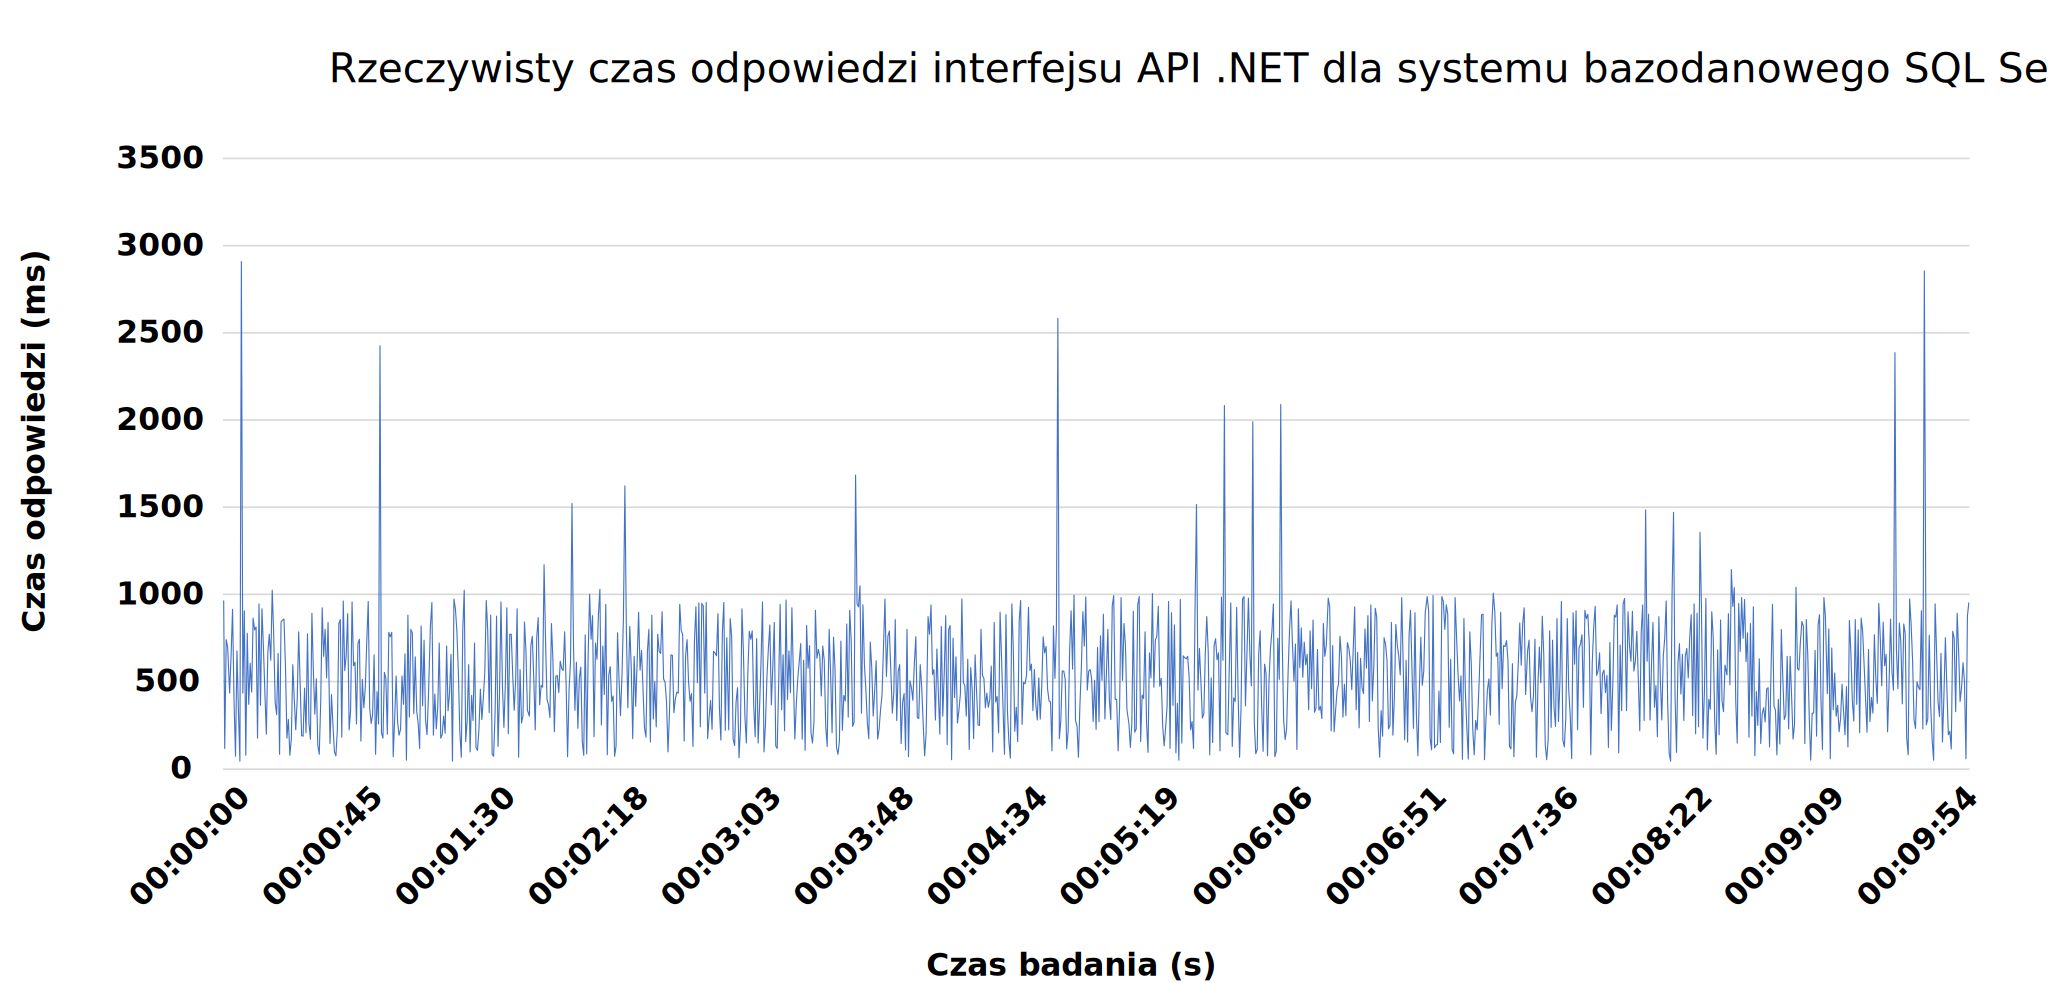
\includegraphics[width=\linewidth]{rys05/testy-funkcjonalne-dotnet.pdf}
    \caption{Czas odpowiedzi na żądanie dla konfiguracji .NET/SQL Server w kontekście testu funkcjonalnego}
    \label{fig:wykres-testy-funkcjonalne-dotnet}
\end{figure}

Na podstawie analogicznych danych, dla każdej pary interfejs API - system bazodanowy, zdefiniowano progi tolerancji oraz frustracji stanowiące punkty odniesienia przy kalkulacji wartości wskaźnika APDEX. Wartości te, ustalono poprzez rosnące posortowanie zbioru czasów odpowiedzi API, a następnie dokonanie symetrycznego podziału dwupunktowego.

Uzyskane przedziały satysfakcji, tolerancji oraz frustracji względem każdego systemu bazodanowego oraz technologii tworzenia API zostały zobrazowane na wykresach \ref{fig:apdex-dotnet} oraz \ref{fig:apdex-nodejs}.

\begin{figure}[ht]
    \centering
     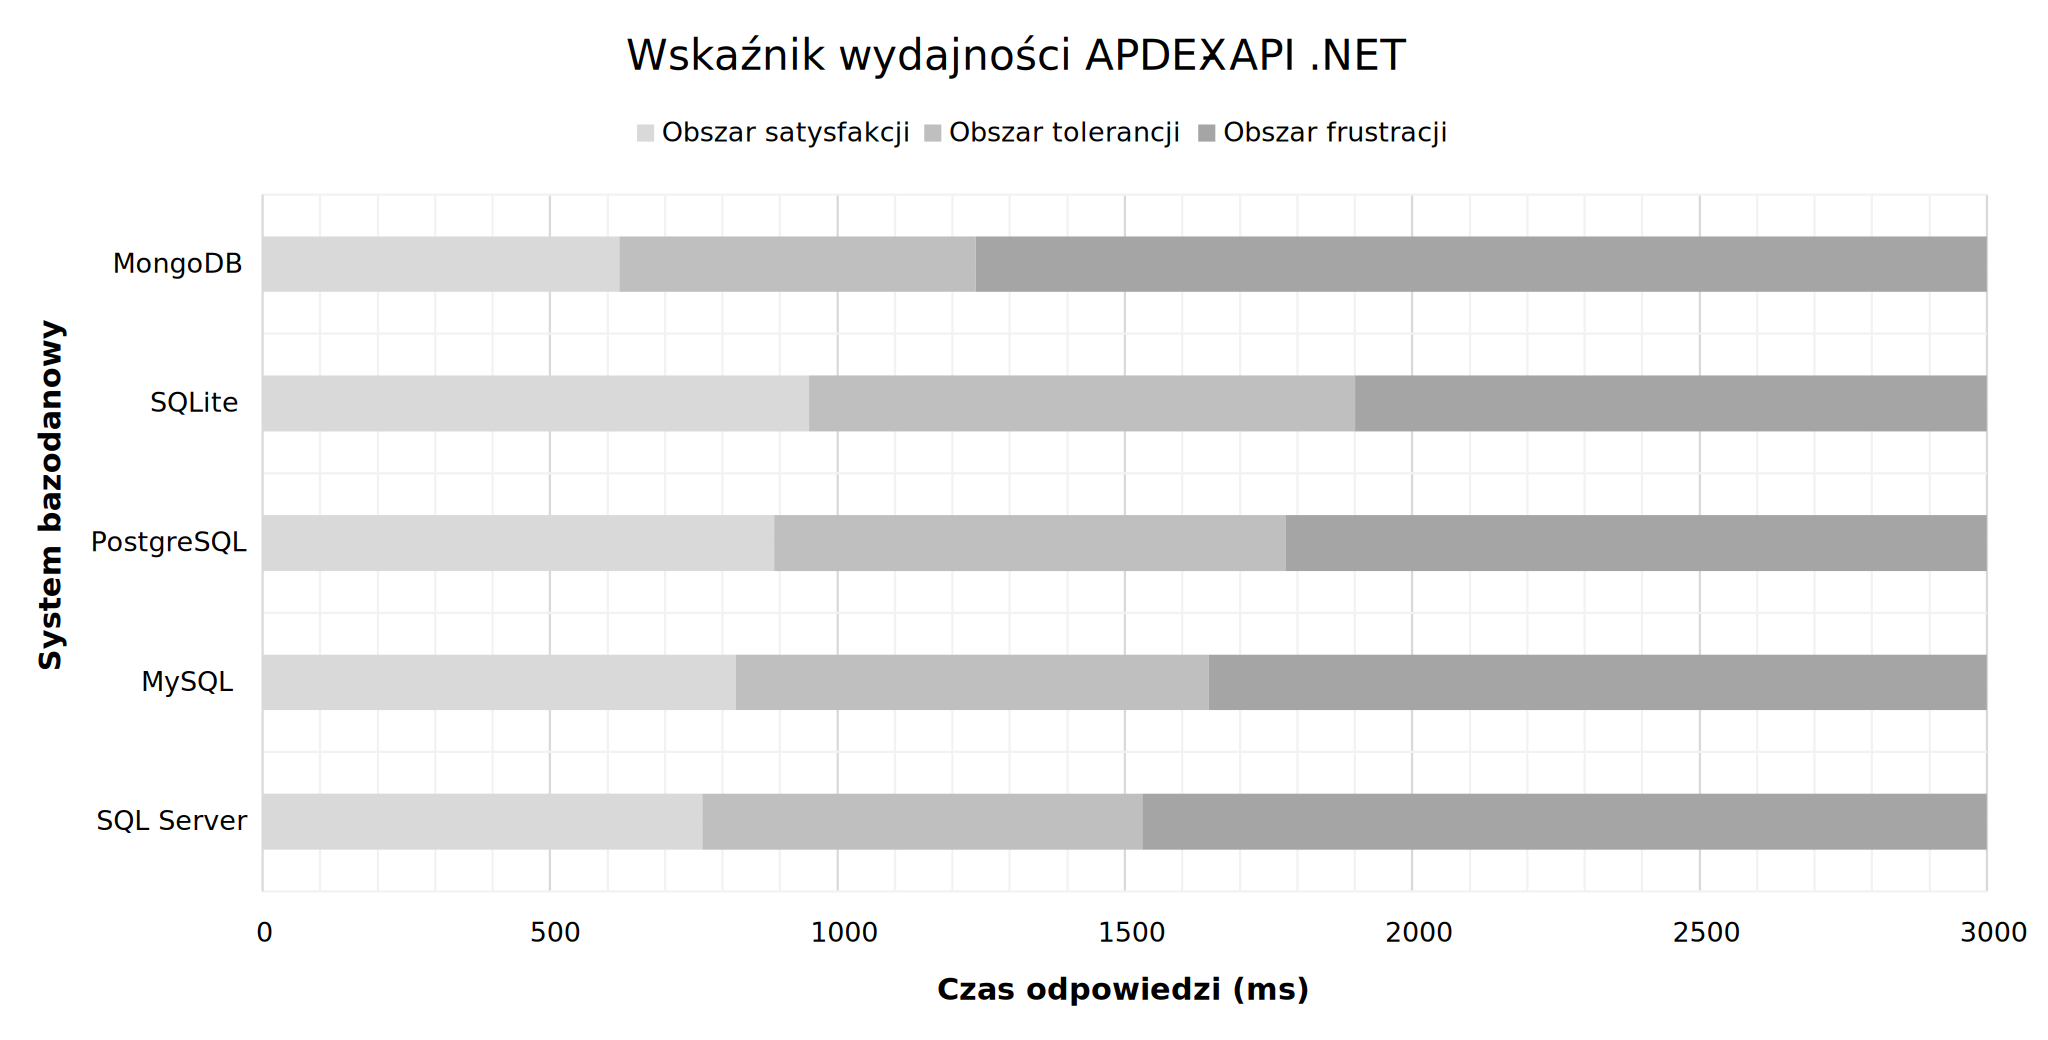
\includegraphics[width=\linewidth]{rys05/apdex-dotnet.pdf}
    \caption{Obszary satysfakcji, tolerancji oraz frustracji wskaźnika APDEX względem poszczególnych systemów bazodanowych dla API zaimplementowanego w C\#}
    \label{fig:apdex-dotnet}
\end{figure}

\begin{figure}[ht]
    \centering
     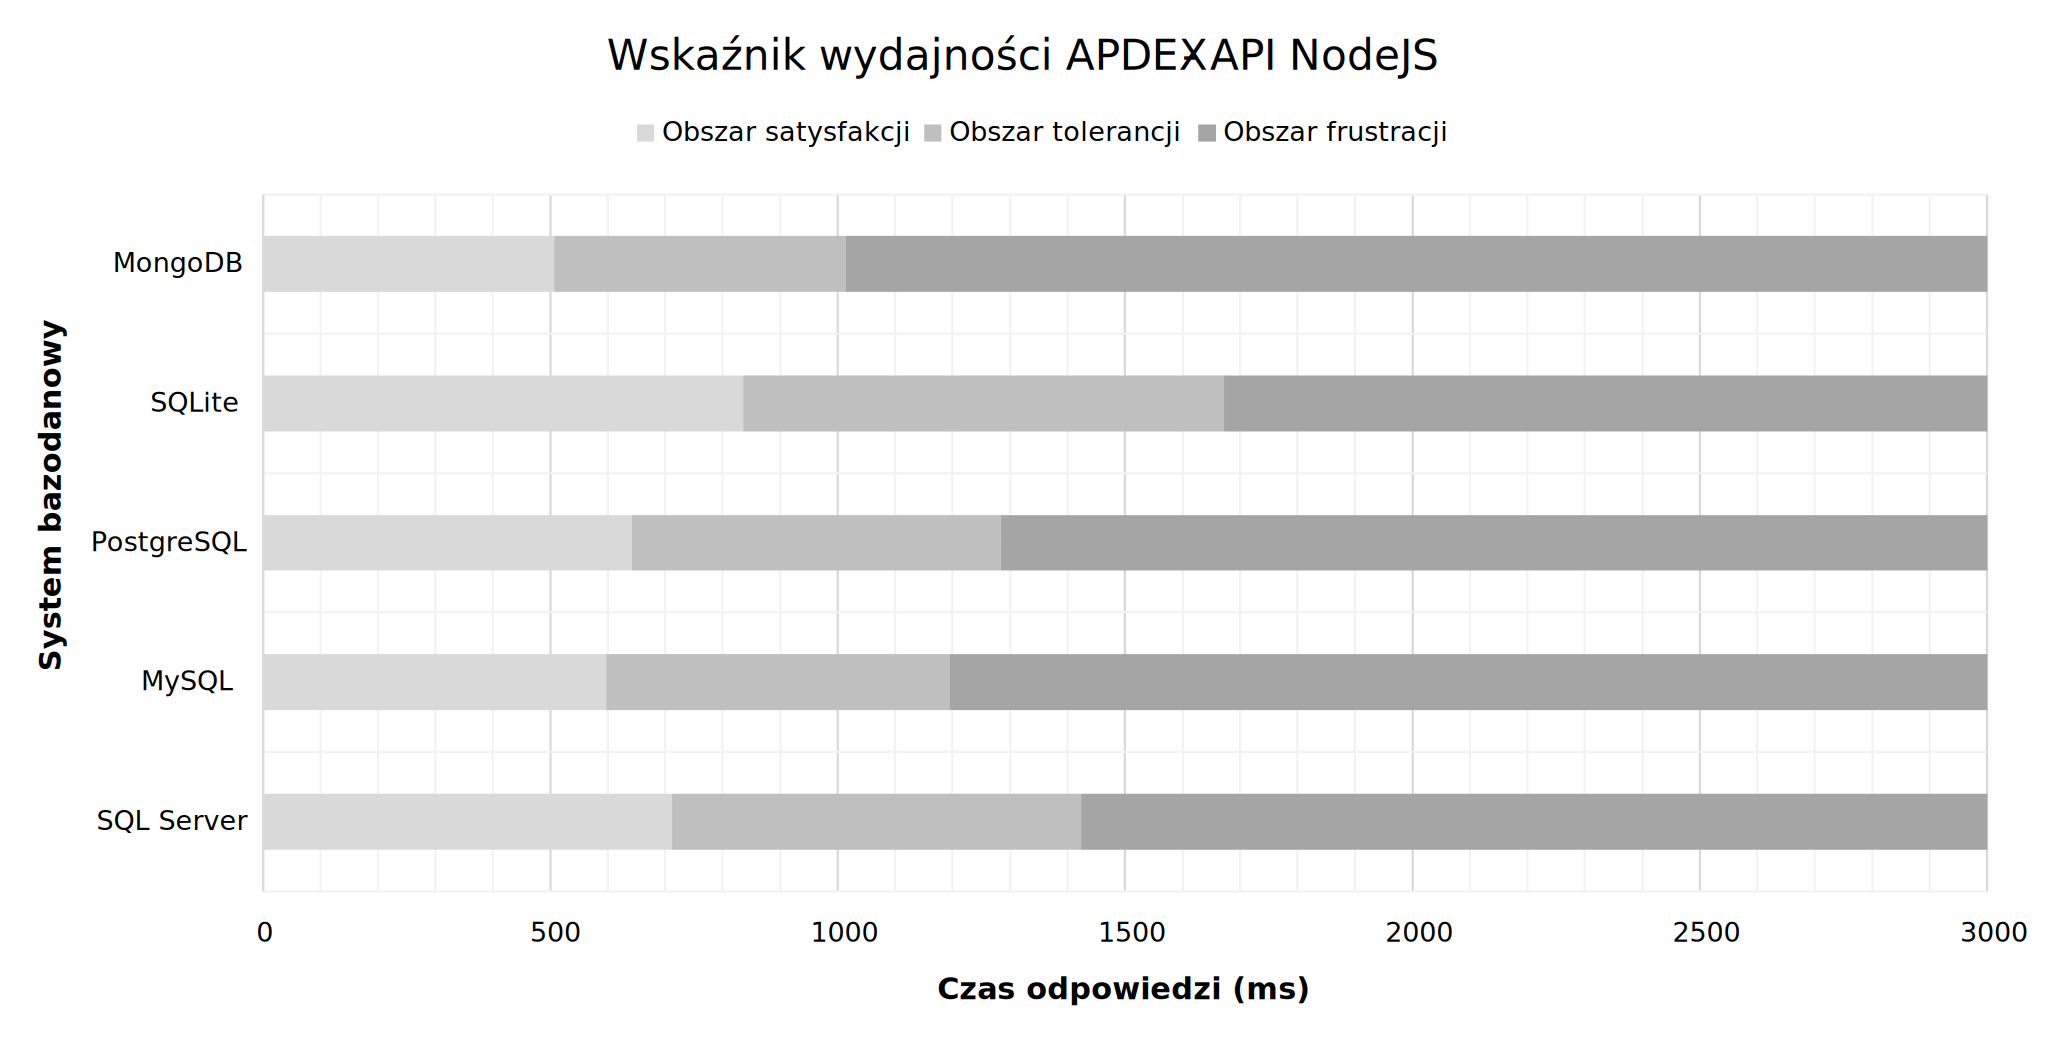
\includegraphics[width=\linewidth]{rys05/apdex-nodejs.pdf}
    \caption{Obszary satysfakcji, tolerancji oraz frustracji wskaźnika APDEX względem poszczególnych systemów bazodanowych dla API zaimplementowanego w JavaScript}
    \label{fig:apdex-nodejs}
\end{figure}


Po spełnieniu warunków początkowych badania zrealizowano faktyczne czynności badawcze. Wykorzystując lokalną topologię fizyczną \ref{sec:lokalne-srodowisko-badawcze-ver-1} rozpoczęto generowanie żądań protokołu hipertekstowego wytwarzanych przez dwa równolegle pracujące hosty sieciowe. Procedura badawcza trwała 20 minut i polegała na stopniowym zwiększaniu liczby współbieżnie pracujących procesów oprogramowania testującego rozpoczynając od jednego procesu a kończąc na pięciu tysiącach. Nowe wątki oprogramowania Apache JMeter uruchamiane były w stałych odstępach czasu, co implikuje niezmienność długości przedziału czasowego pracy w obrębie ustalonej liczby wątków. Czas ten, wynosi 240ms. Przy uwzględnieniu minimalnej zaobserwowanej średniej wartości natężenia generowanych żądań, wynoszącej 152 zapytania w ciągu sekundy, liczebność zbioru próbek czasu zapytania w odniesieniu do dowolnego z 4990 poziomów przyrostu ruchu wyniosła co najmniej 36 elementów. Pierwsze 10 poziomów dotyczących liczby klientów generujących komunikaty nie pozwoliło na zarejestrowanie co najmniej 30 próbek, przez co elementy te, nie były brane pod uwagę w czasie opracowywania uzyskanych wyników. Opisane w niniejszym akapicie czynności zostały wykonane względem interfejsów programowania aplikacji wykorzystujących porównywane technologie, uwzględniając komunikację z każdym z pięciu systemów bazodanowych.

Na wykresach \ref{fig:response-mtc-1} a) do \ref{fig:response-mtc-1} j) zaprezentowano uśrednione względem liczby pracujących wątków, czasy odpowiedzi na żądanie generowane w kierunku ewaluowanych interfejsów API.

\begin{figure}[htb]
  \centering
	\begin{tabular}{@{}ll@{}}
    a) & b) \\
    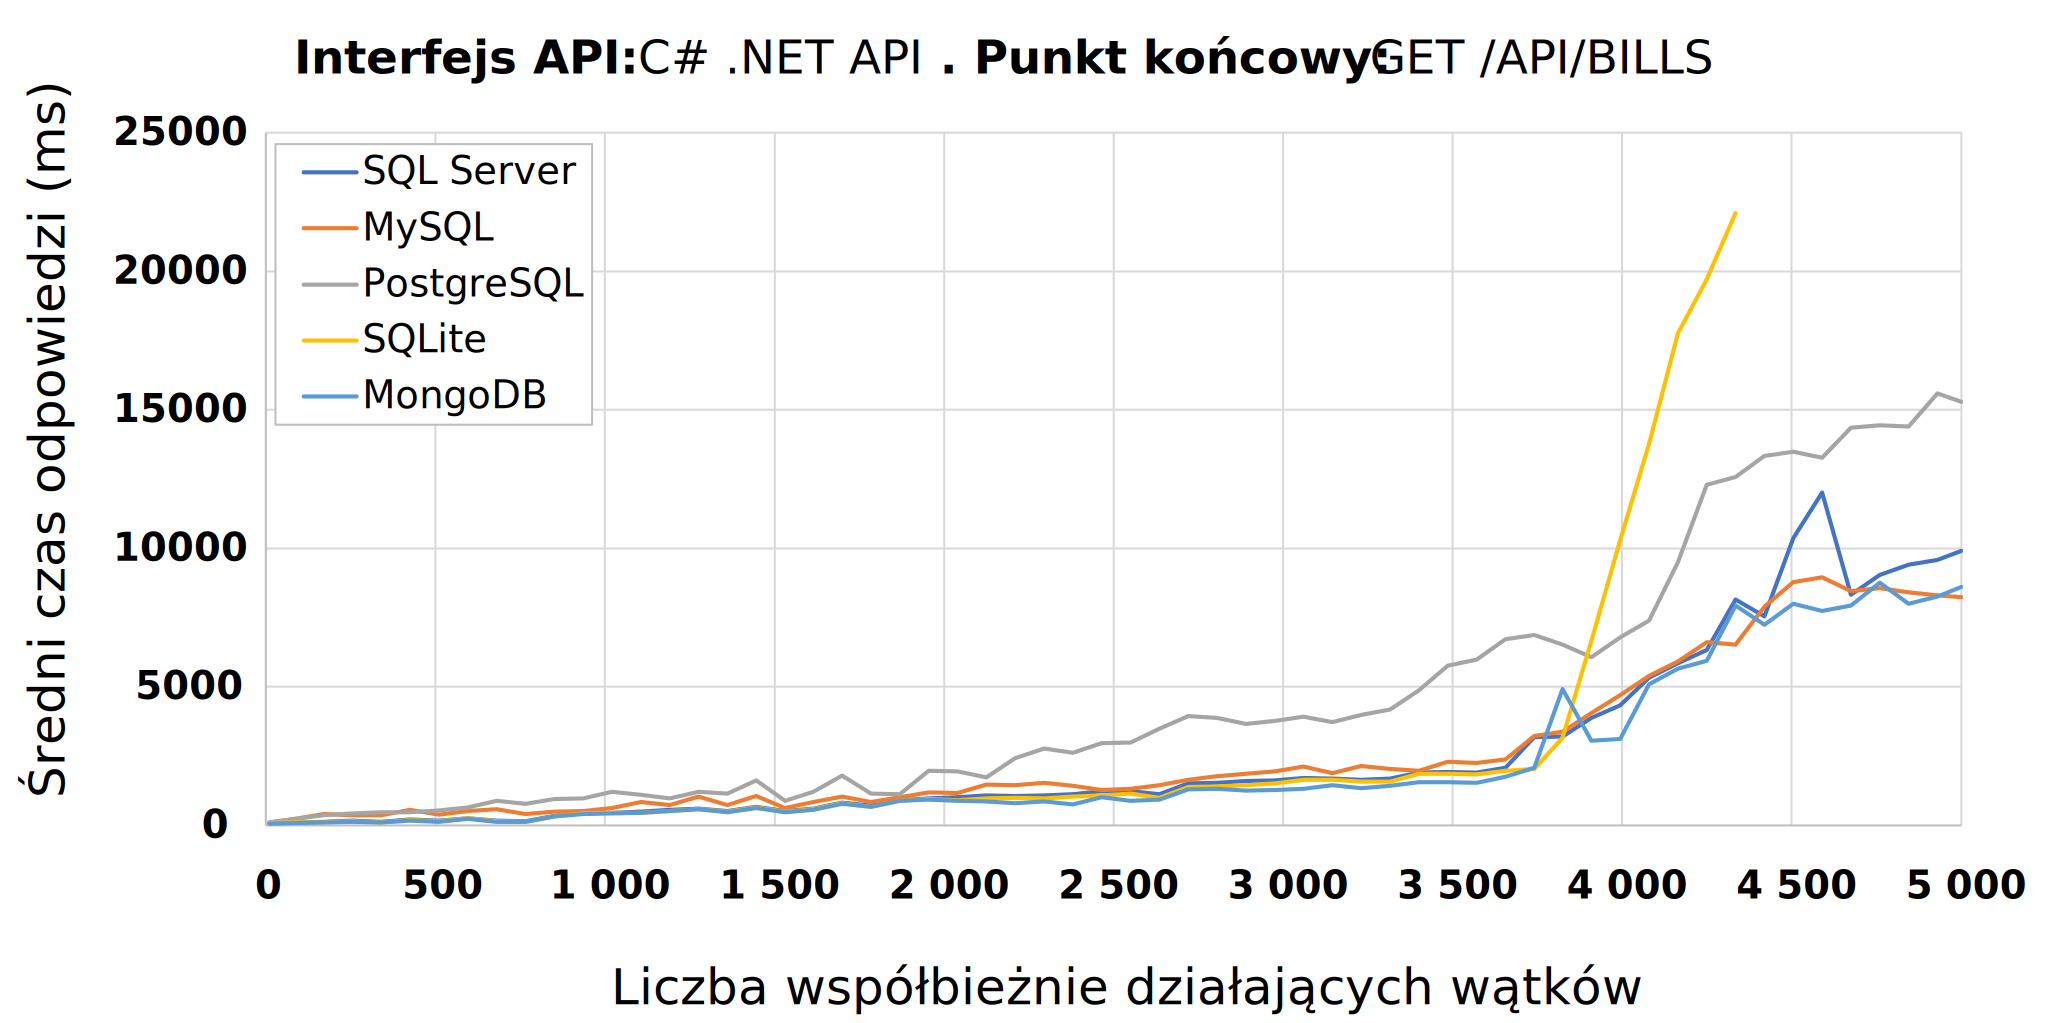
\includegraphics[width=0.49\textwidth]{rys05/response-dotnet-fetchAllBills.pdf} & 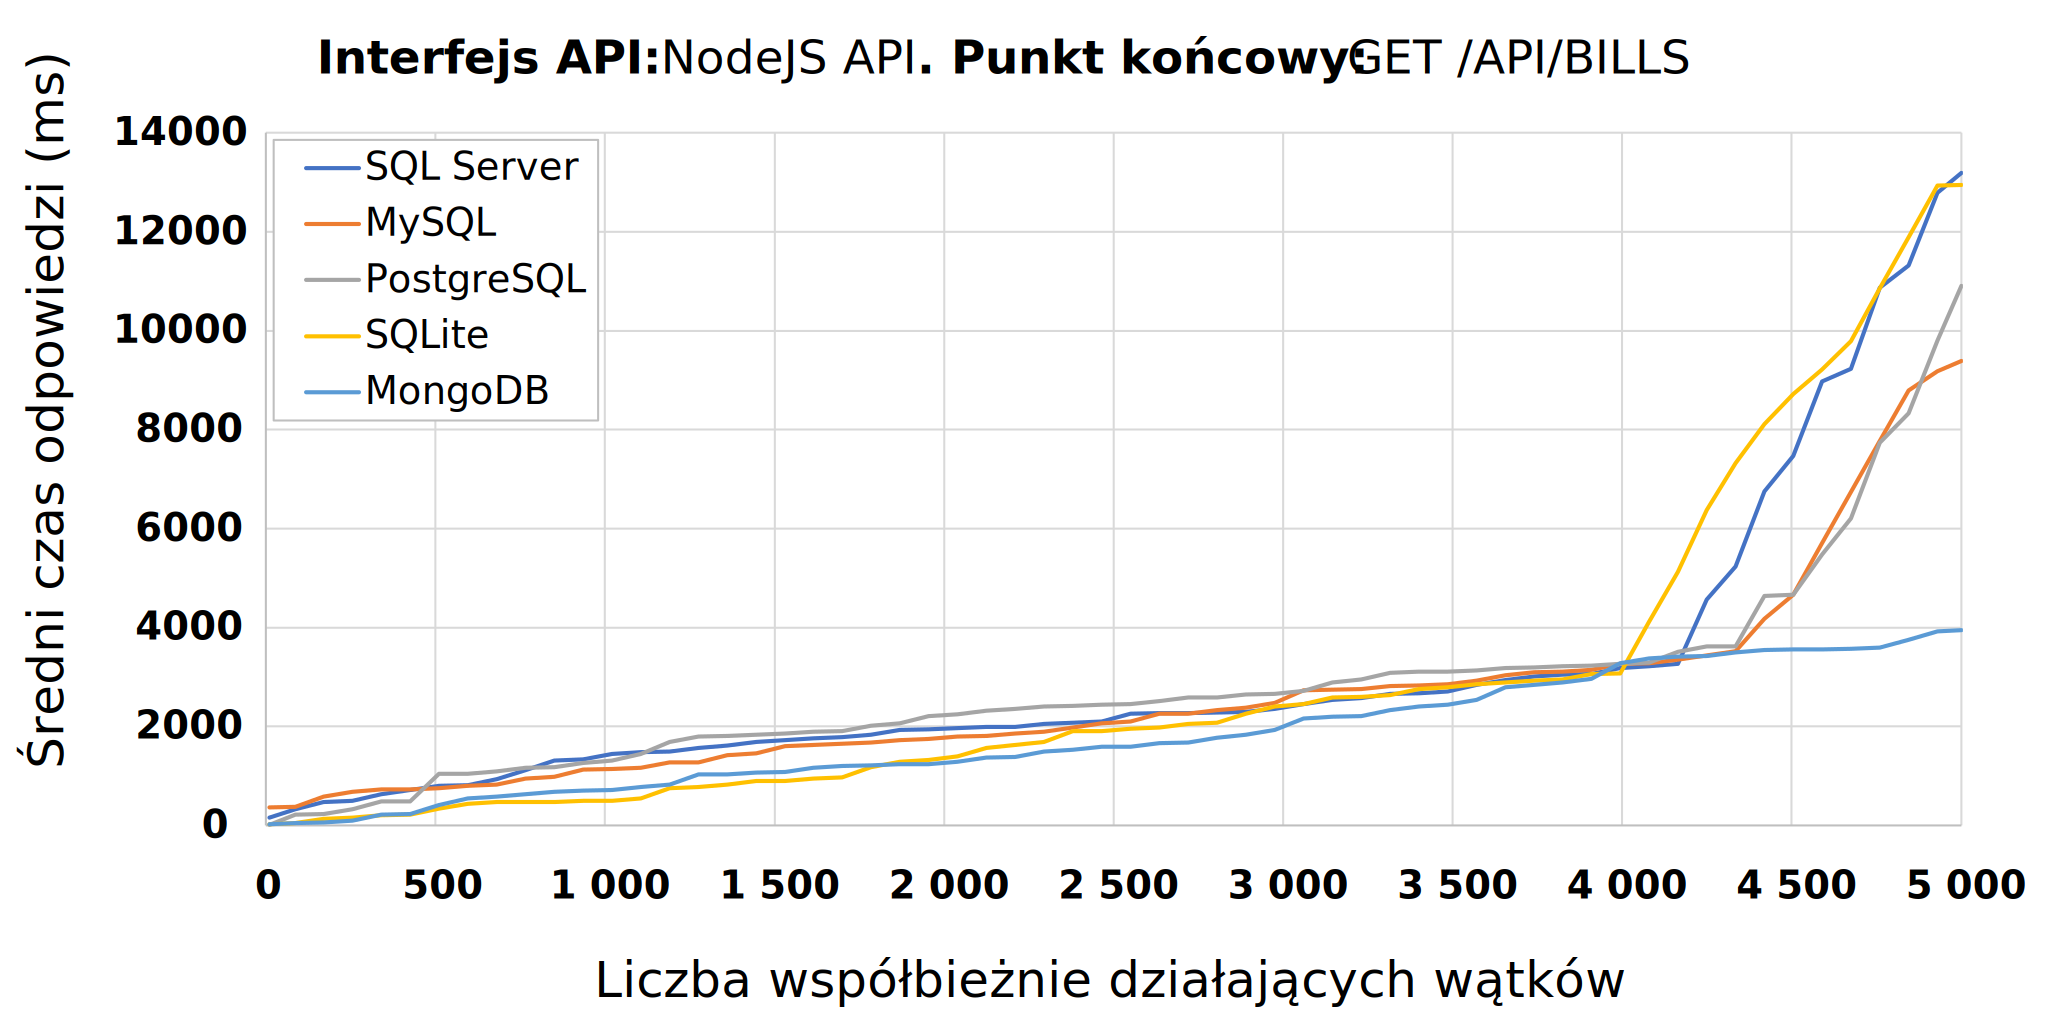
\includegraphics[width=0.49\textwidth]{rys05/response-nodejs-fetchAllBills.pdf} \\
    c) & d) \\
    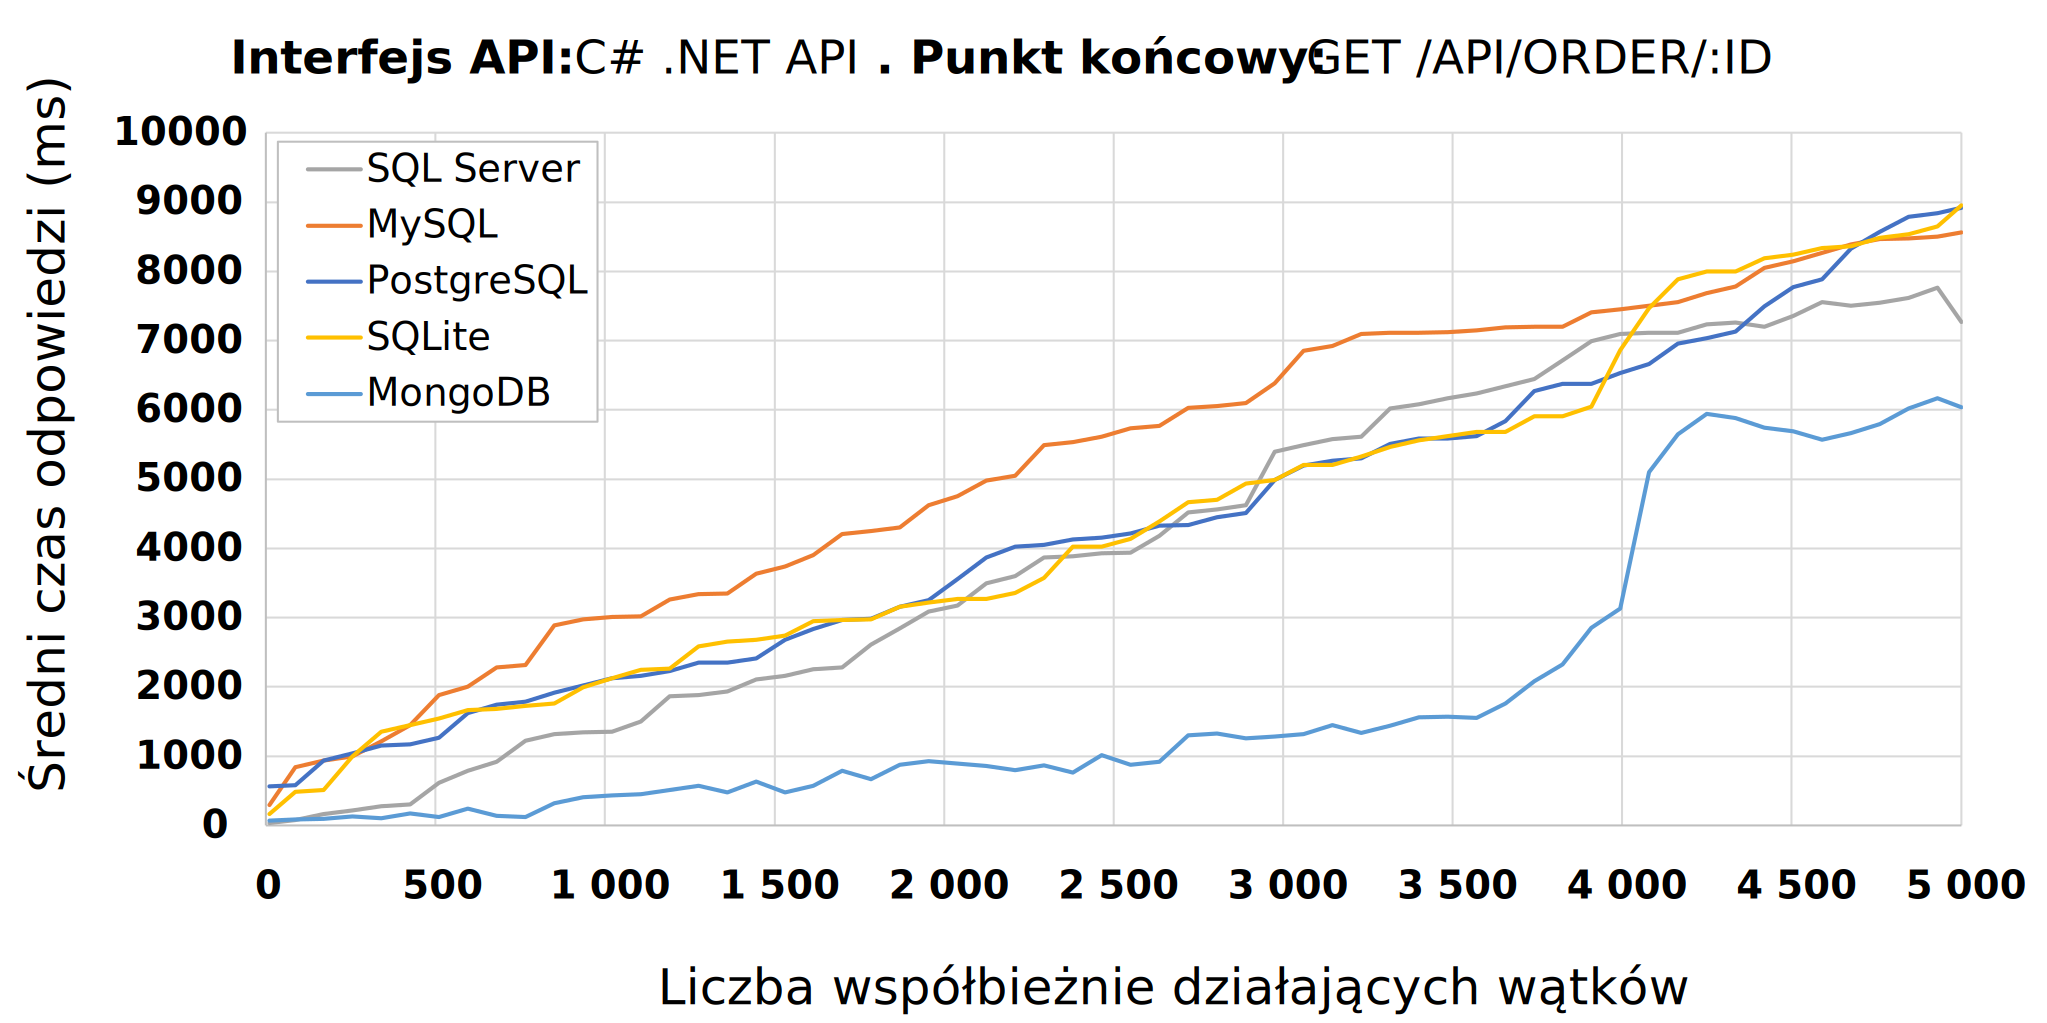
\includegraphics[width=0.49\textwidth]{rys05/response-dotnet-getSingleOrder.pdf} & 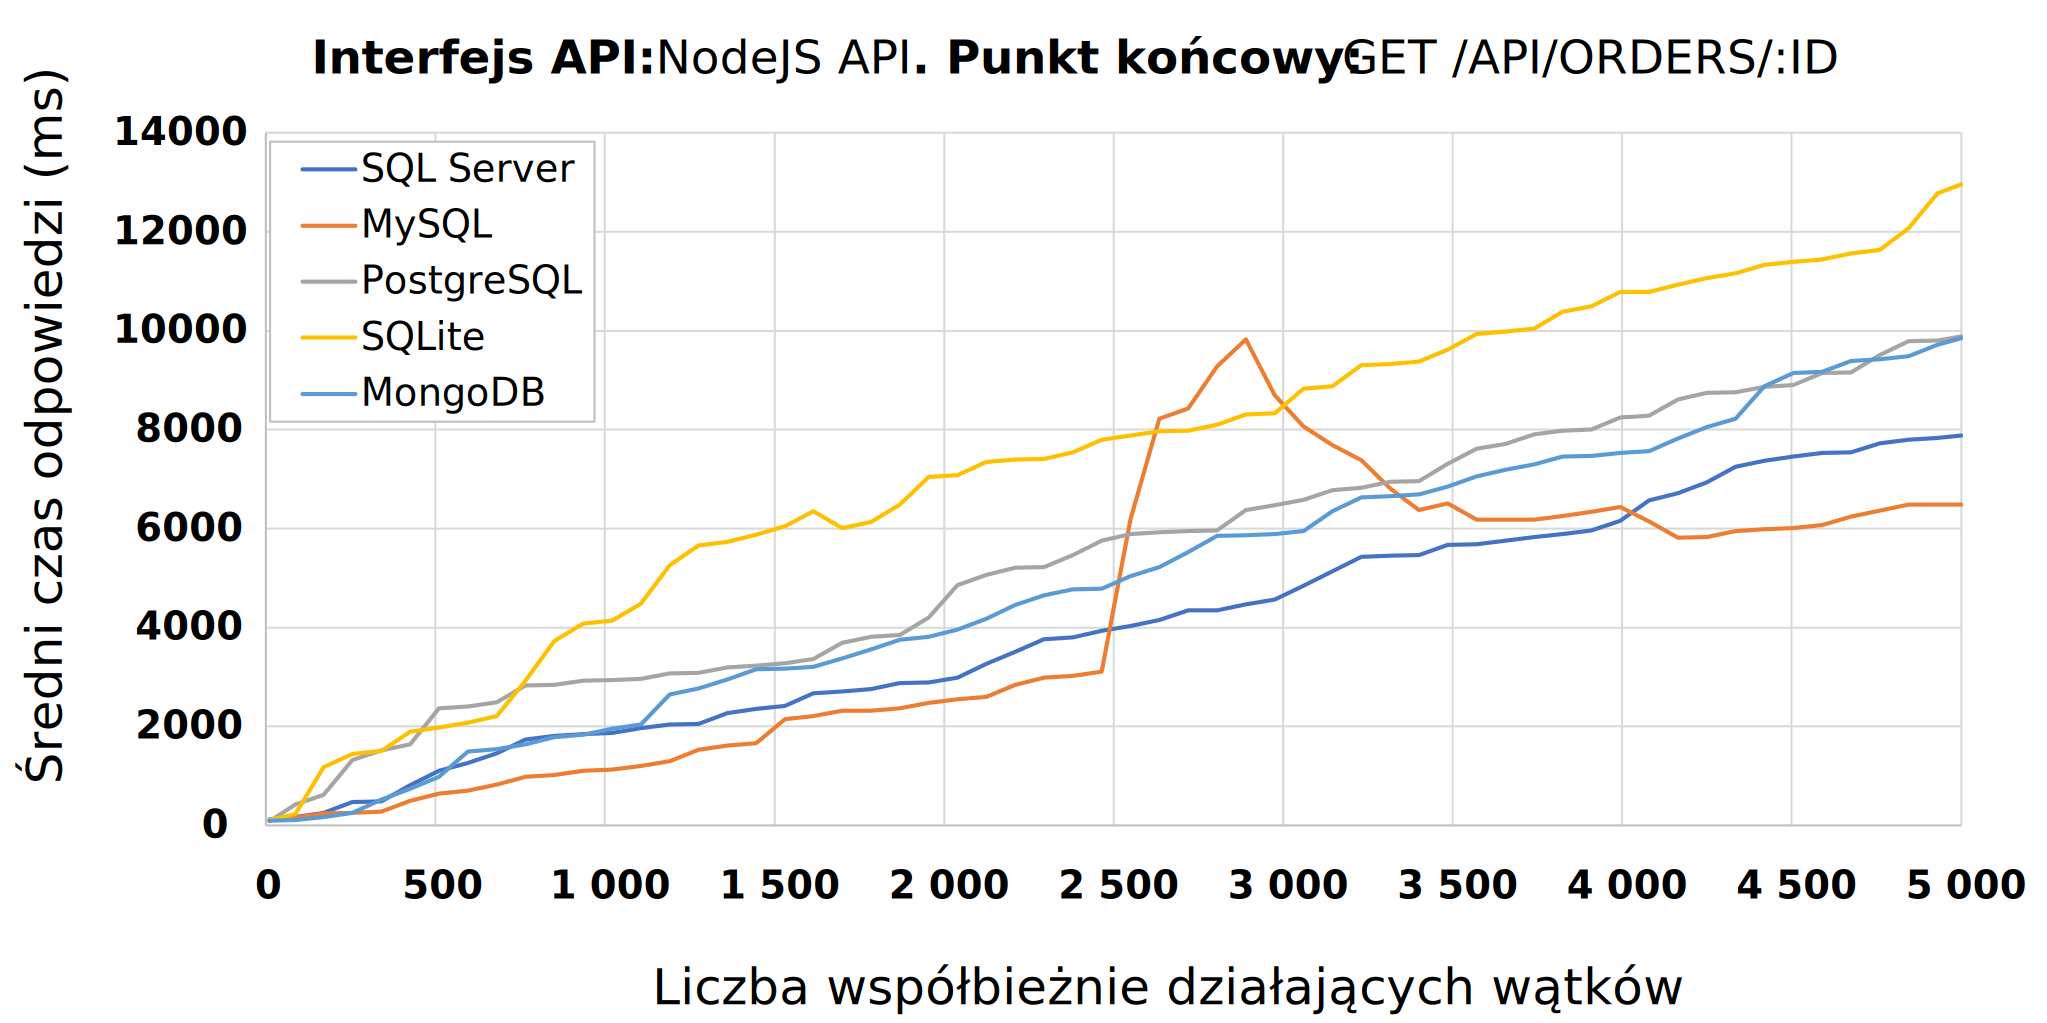
\includegraphics[width=0.49\textwidth]{rys05/response-nodejs-getSingleOrder.pdf} \\
    e) & f) \\
    \includegraphics[width=0.49\textwidth]{rys05/response-dotnet-addProduct.pdf} & 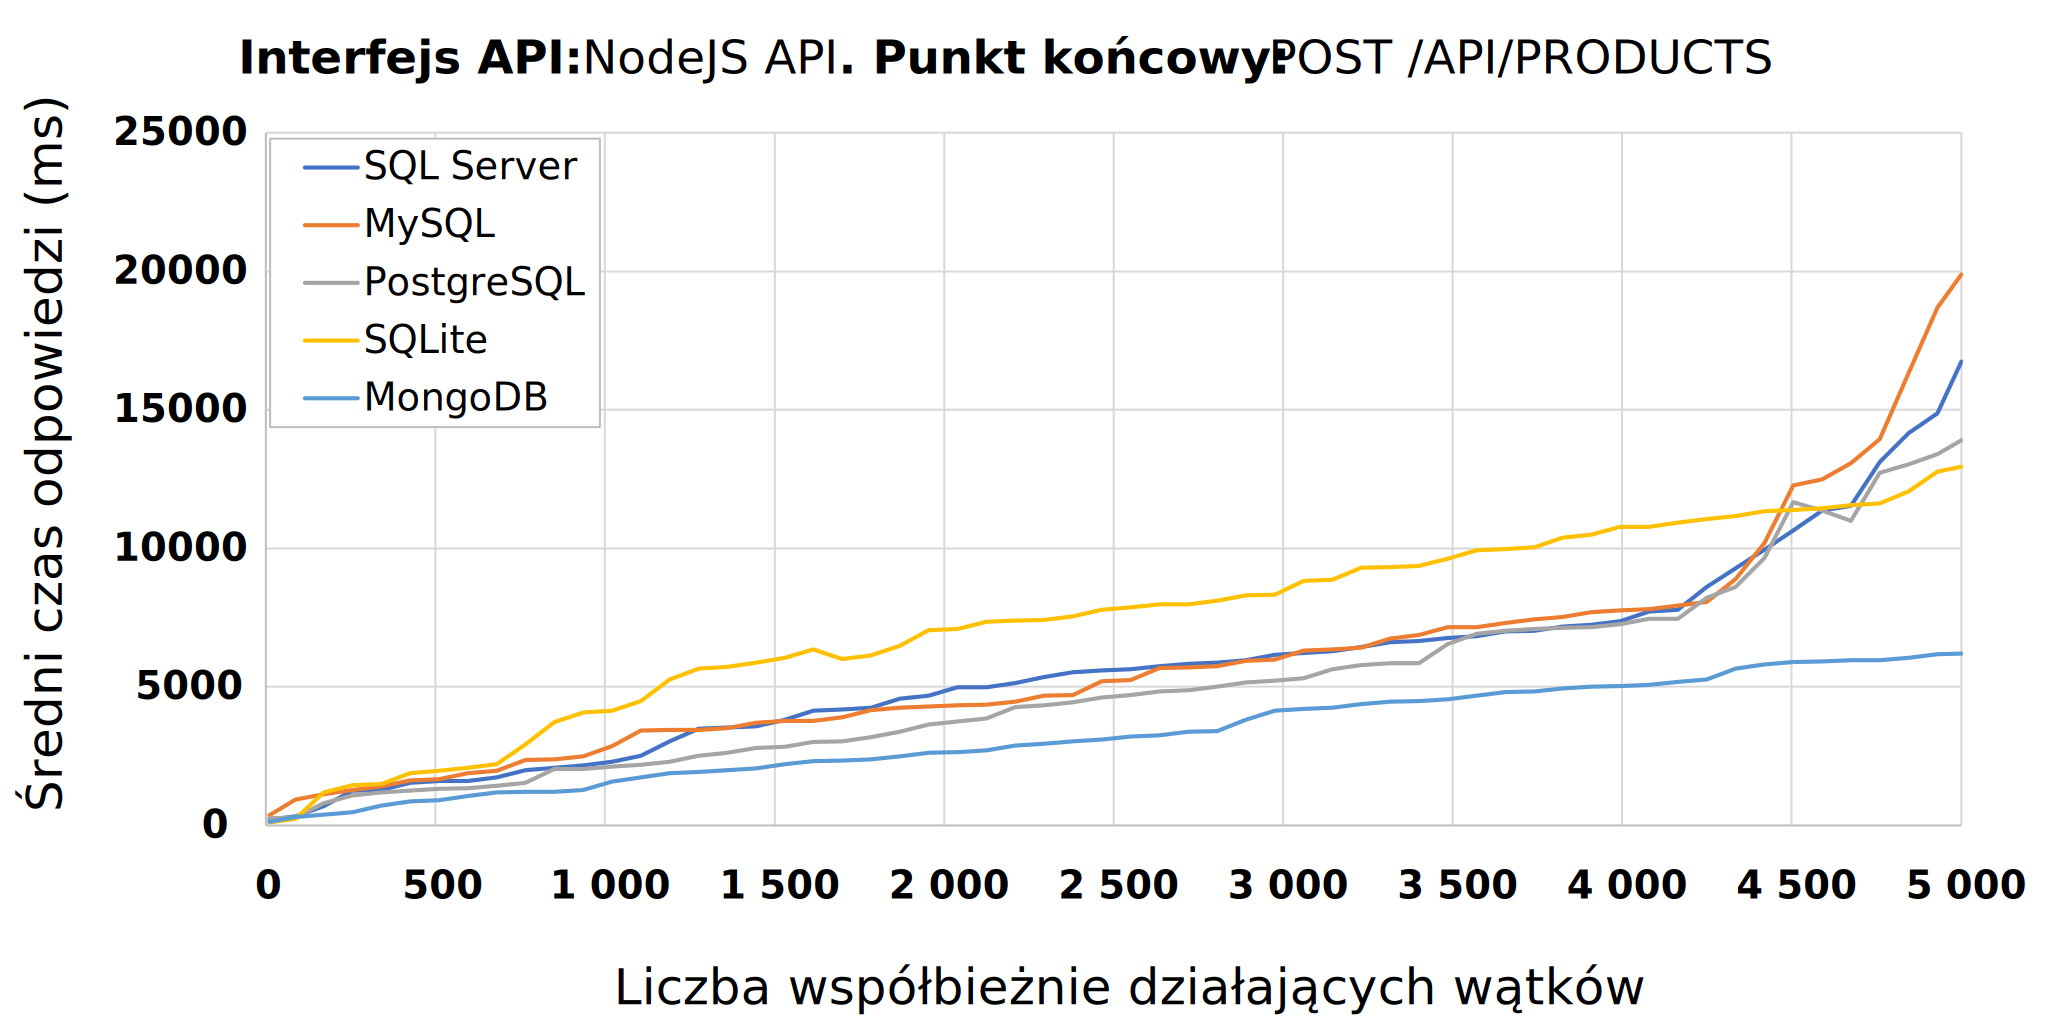
\includegraphics[width=0.49\textwidth]{rys05/response-nodejs-addProduct.pdf} \\
    g) & h) \\
    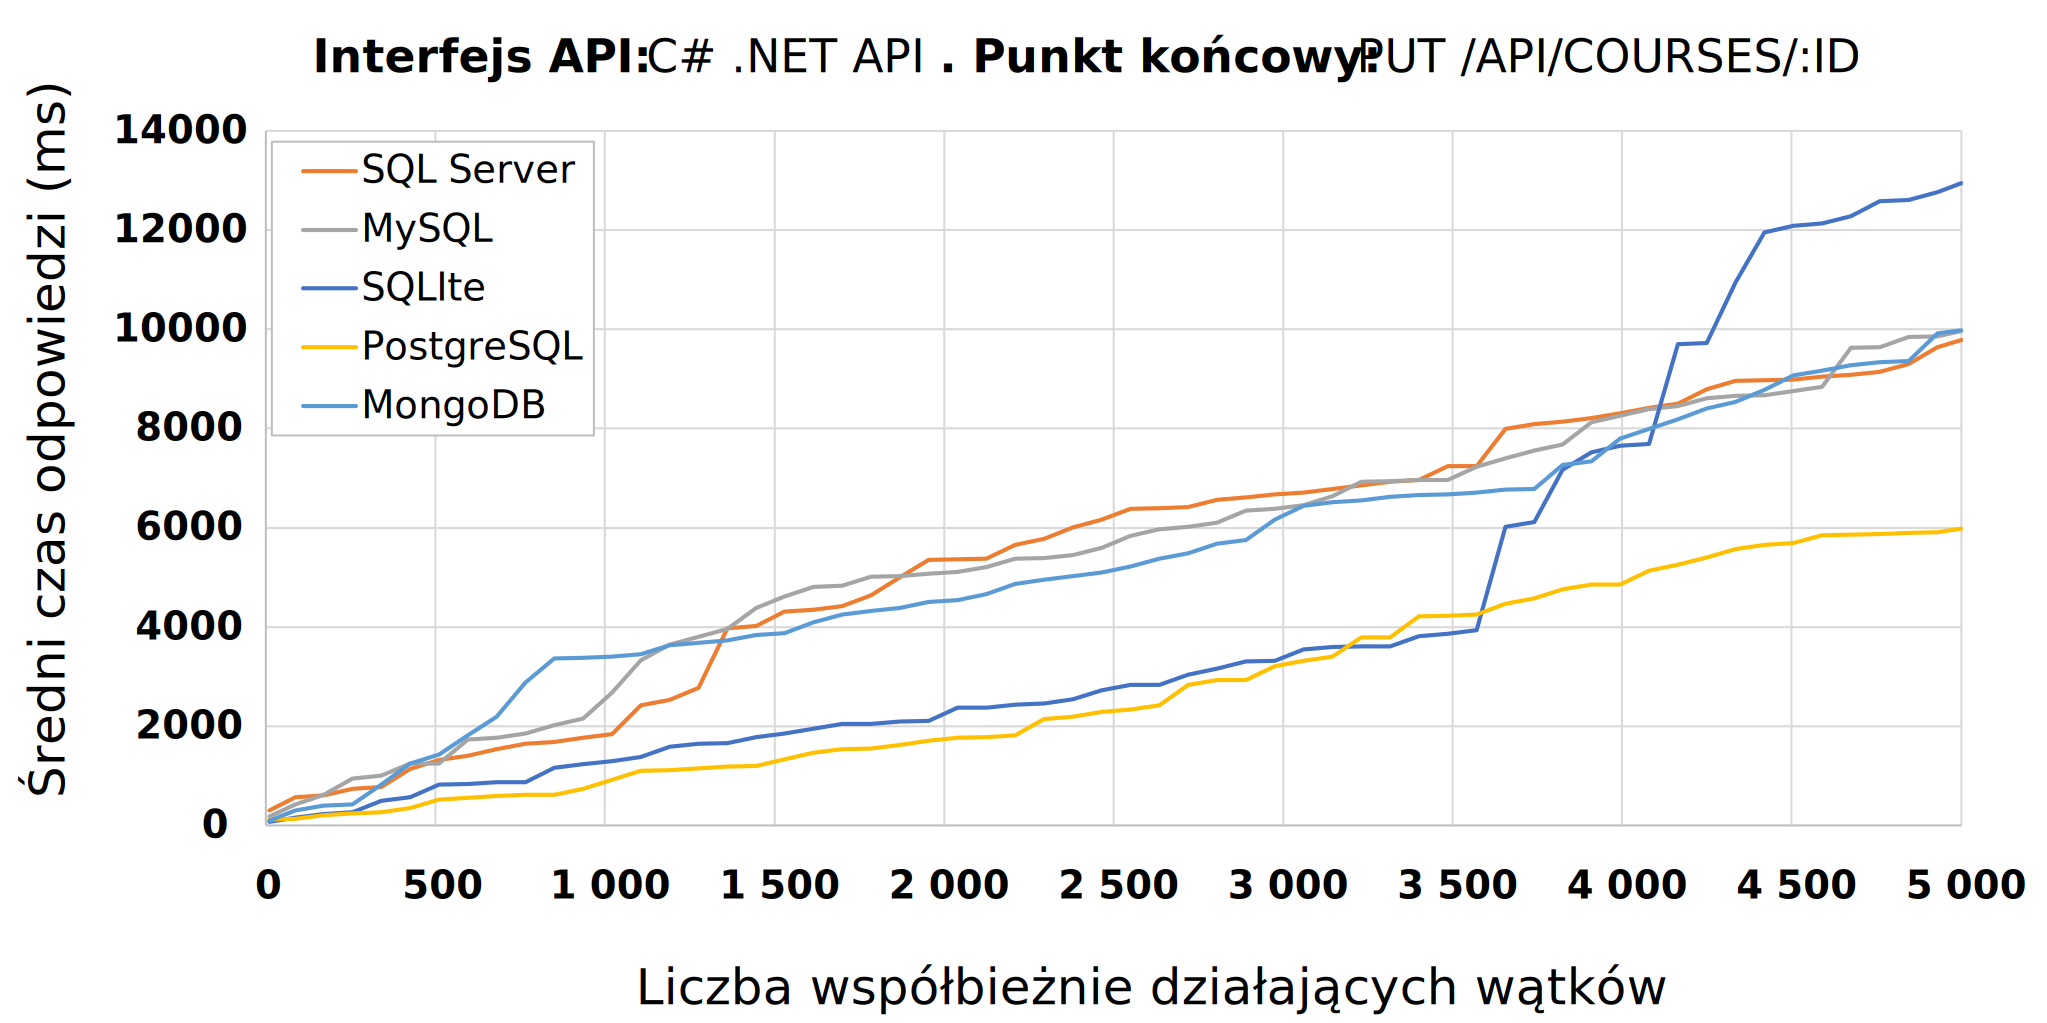
\includegraphics[width=0.49\textwidth]{rys05/response-dotnet-updateCourse.pdf} & 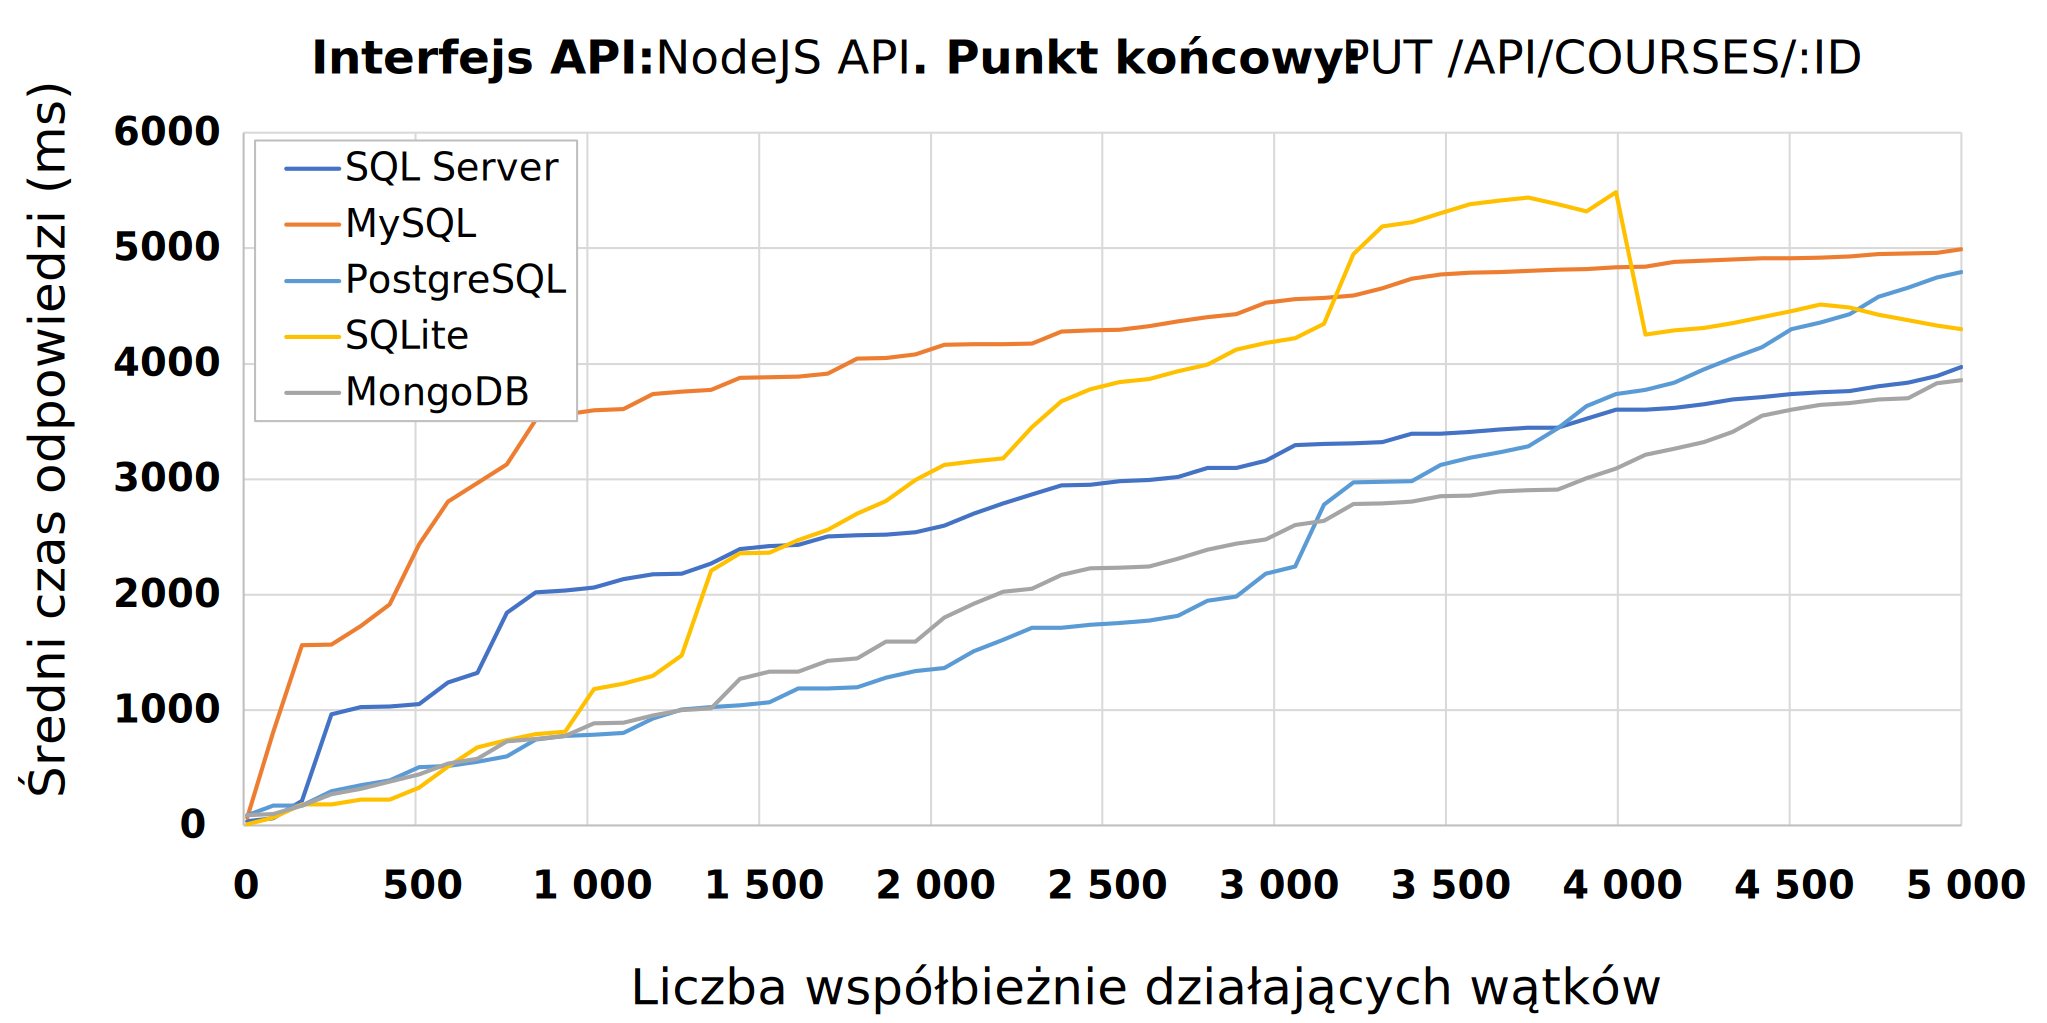
\includegraphics[width=0.49\textwidth]{rys05/response-nodejs-updateCourse.pdf} \\
    i) & j) \\
    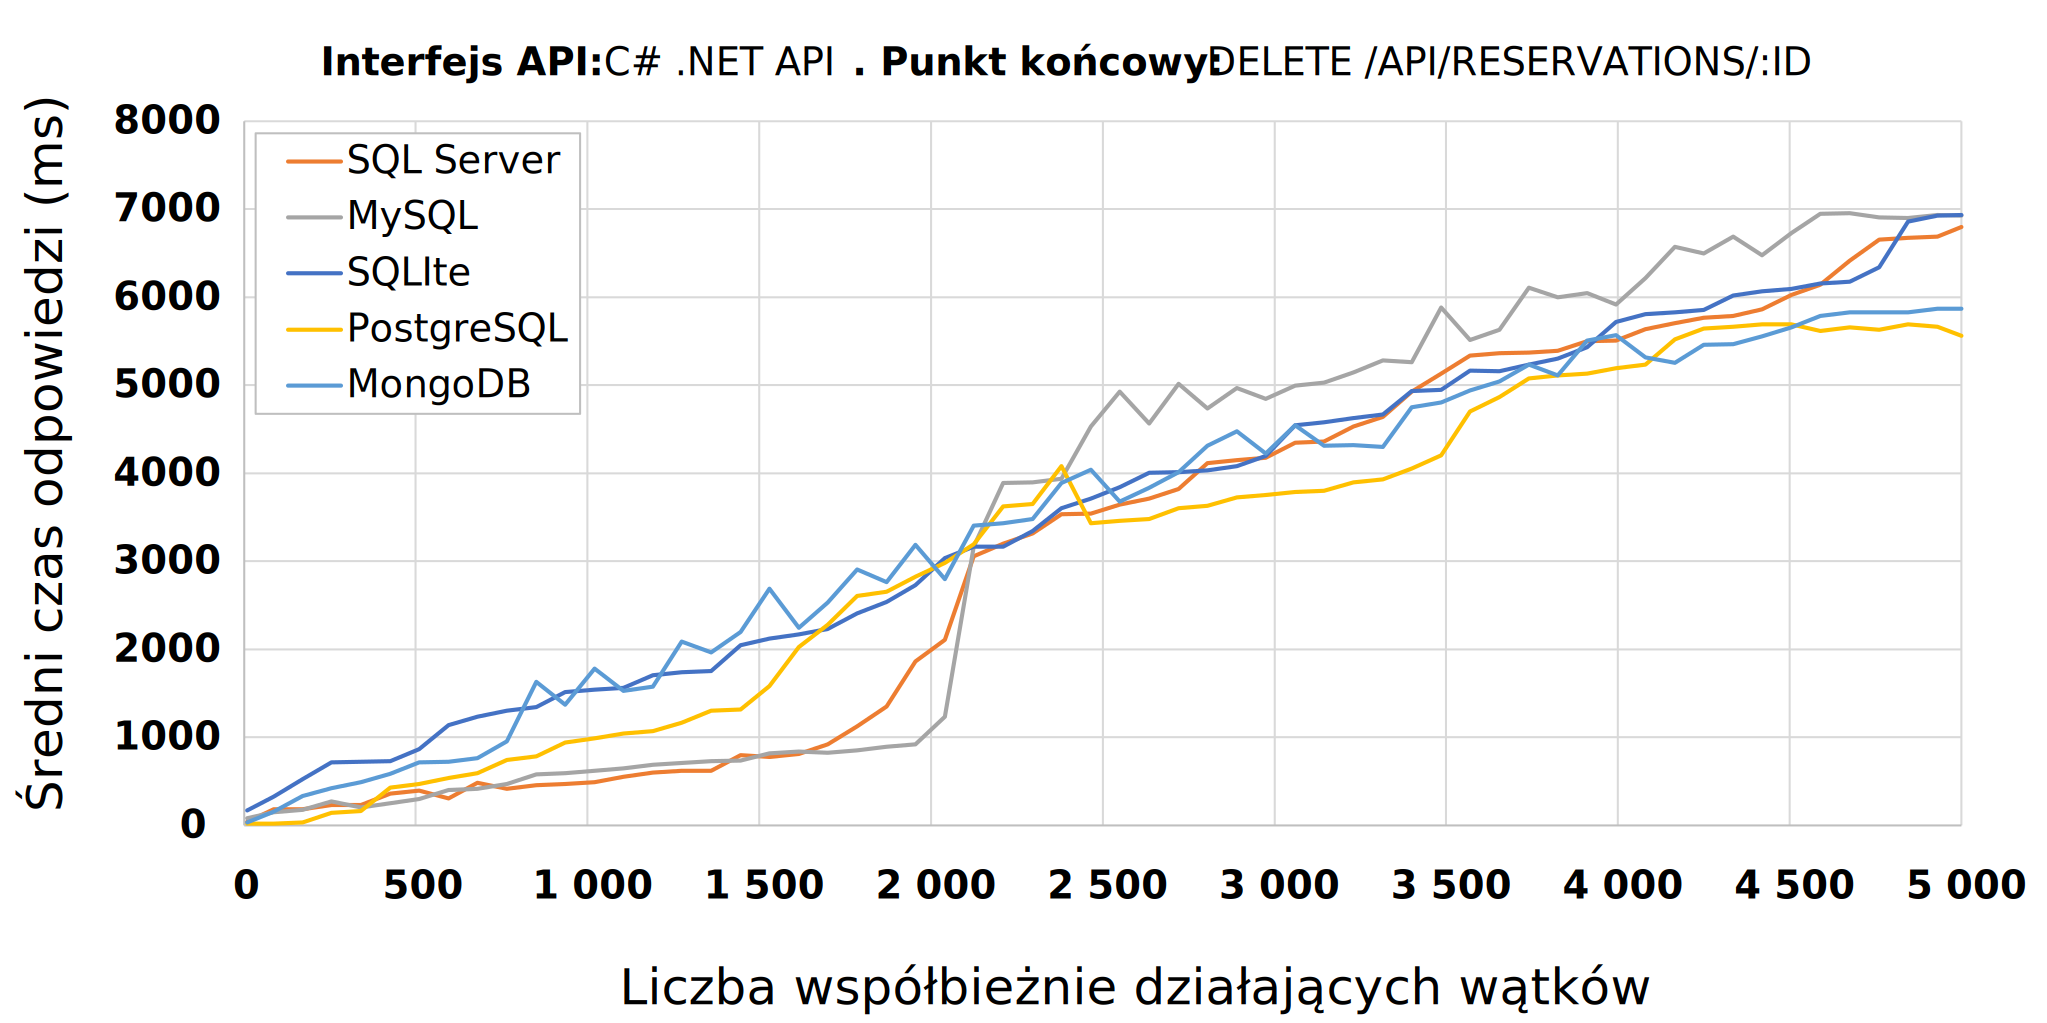
\includegraphics[width=0.49\textwidth]{rys05/response-dotnet-deleteReservation.pdf} & 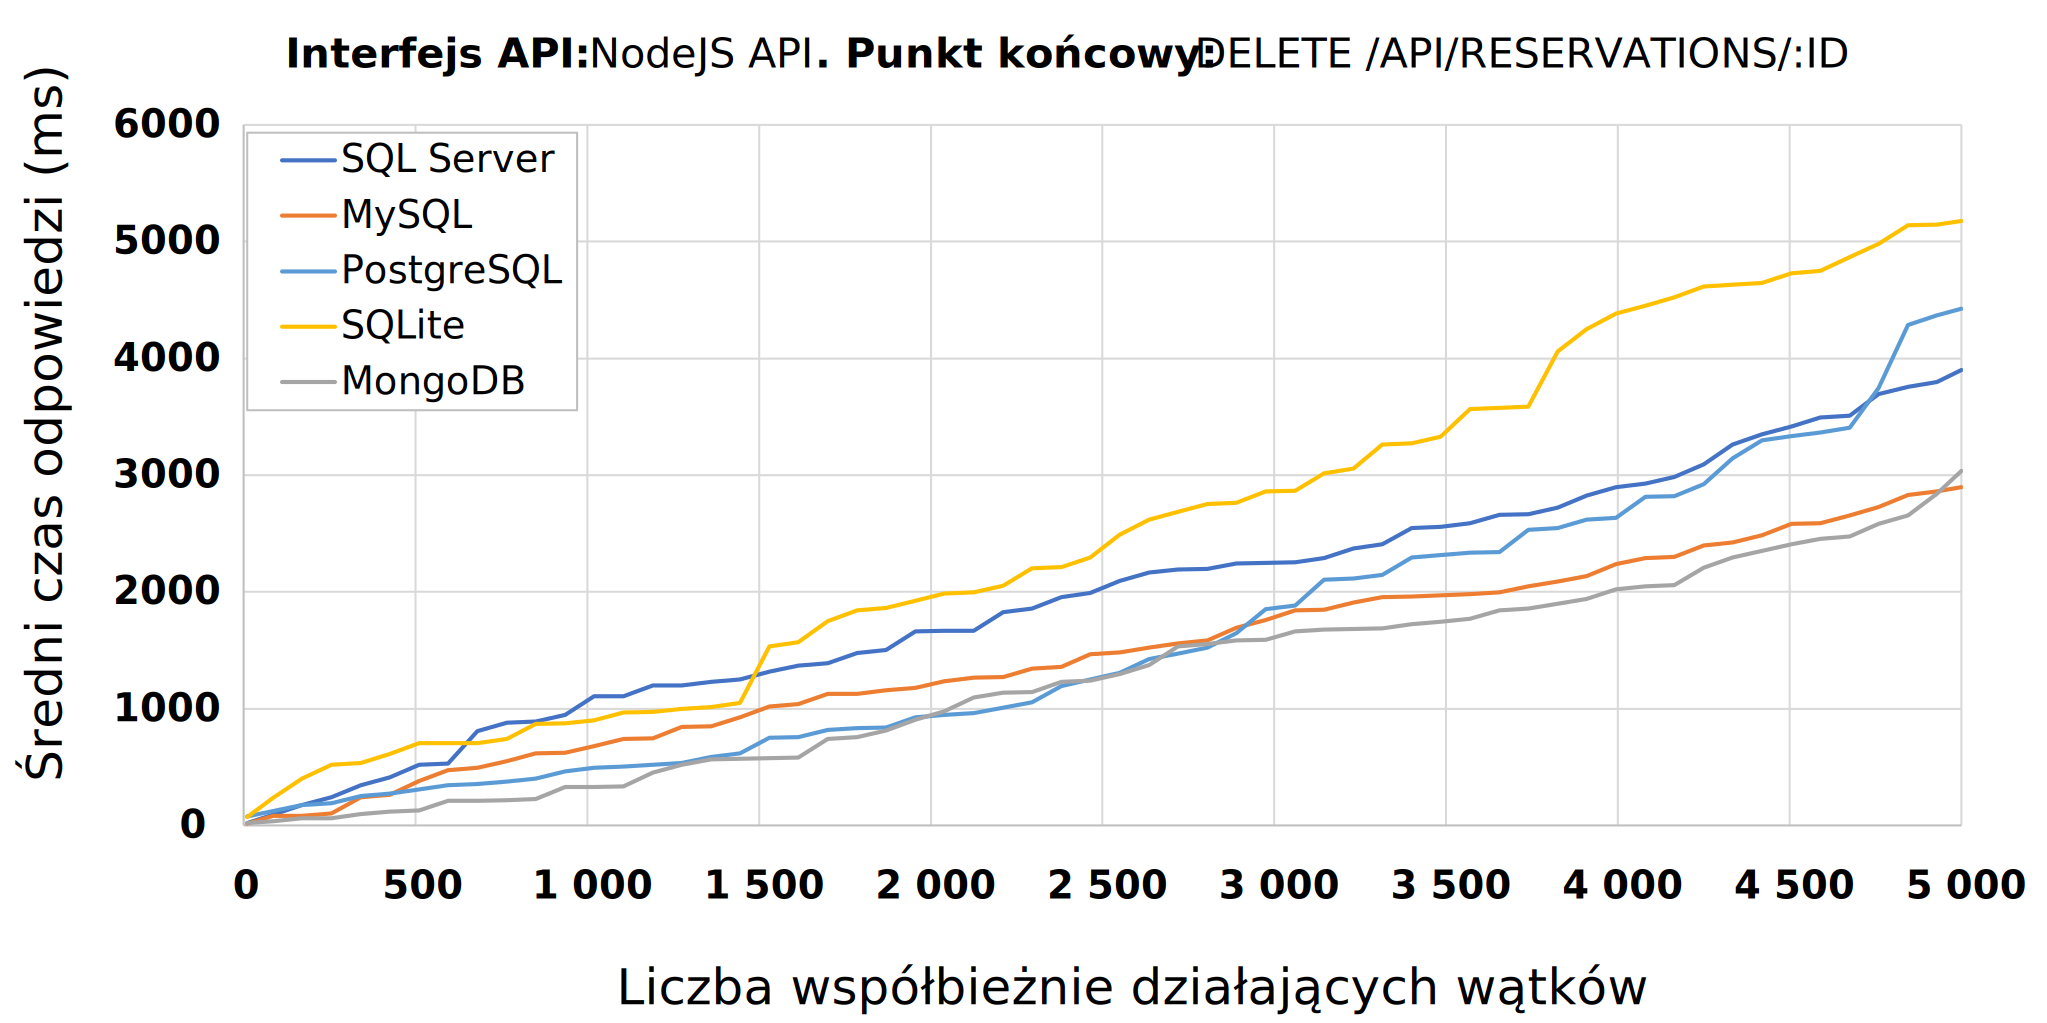
\includegraphics[width=0.49\textwidth]{rys05/response-nodejs-deleteReservation.pdf} \\
	% jezeli obraki sa rownej wysokosci, mozna je wyrownac do gory stosujac vtop jak nizej
	% \vtop{\vskip-2ex\hbox{{\includegraphics[width=0.475\textwidth]{rys05/beta1}}}} &
	% \vtop{\vskip-2ex\hbox{{\includegraphics[width=0.475\textwidth]{rys05/alfa1}}}}  \caption{Wyznaczanie trajektorii lotu rakiety: 
	\end{tabular}
  \caption{Średnie czasy odpowiedzi na żądanie względem liczby procesów generujących oraz systemu bazodanowego}
  \label{fig:response-mtc-1}
\end{figure}

Zauważyć należy znaczącą różnicę czasów odpowiedzi na żądanie w kontekście pobierania kolekcji encji bazodanowych. Różnica ta, faworyzuje rozwiązanie oparte o język JavaScript oraz platformę uruchomieniową NodeJS w odniesieniu do czterech z pięciu wykorzystywanych systemów baz danych. Wyjątkiem jest tutaj technologia SQL Server, która pozwalała na bardziej sprawne obsługiwanie zapytań poprzez komunikację z usługą sieciową implementowaną w języku C\#. Ponadto, w obrębie zakresu od 3500 do 4500 współbieżnie pracujących wątków generowania zapytań, zaobserwować można nagłe wzrosty czasów odpowiedzi na żądanie. Eskalacja wartości tego parametru związana jest w tym przypadku z osiągnięciem limitu możliwości obsługi zapytań przychodzących do wybranej bazy danych. Limit ten, nie musi być związany z infrastrukturą ani oprogramowaniem serwera. Ograniczenie możliwości wynikać może z zastosowania domyślnych parametrów połączenia pomiędzy usługami. Wpływ wprowadzenia usprawnień wydajnościowych, w tym dostosowania parametrów połączenia oraz określenia puli połączeń, zweryfikowany zostanie w badaniu \ref{sec:cqrs-and-database-improvements}.  

Odwołując się do pozostałych rodzajów wykonywanych operacji, zauważyć można wydatnie niższy czas obsługi żądania dodającego encję, wygenerowanego z kierunku rozwiązania opartego o technologię .NET. W przypadku czynności aktualizacji oraz usuwania encji z kolei, znaczną przewagę posiada ekosystem JavaScript wraz ze środowiskiem NodeJS.

Przedstawione powyżej wyniki nie dostarczają jednakże pełnego obrazu faktycznej wydajności ewaluowanych usług. Należy pamiętać, że uzyskana odpowiedź na żądanie nie musi być zawsze pozytywna, przez co nie zawsze niesie ona ze sobą informacje pożądaną dla klienta. Na wykresach \ref{fig:response-with-errors} a) oraz \ref{fig:response-with-errors} b) zestawiono ze sobą informacje o średnim czasie odpowiedzi na żądanie, a także o procencie żądań zakończonych niepomyślnie. Poprzez niepomyślne zakończenie żądania, rozumiano zarówno uzyskanie odpowiedzi o niepoprawnym kodzie i treści ciała, jak i zgłoszenie wyjątku protokołu hipertekstowego związanego z odmową aplikacji względem realizacji zapytania. Choć zobrazowano tu tylko i wyłącznie przypadek pojedynczej operacji oraz jednego systemu bazodanowego, analogiczne zachowanie zaobserwować można dla wszystkich pozostałych operacji i jest ono specyficzne dla interfejsu programowania aplikacji. 

\begin{figure}[htb]
    \centering
      \begin{tabular}{@{}ll@{}}
      a) & b) \\
      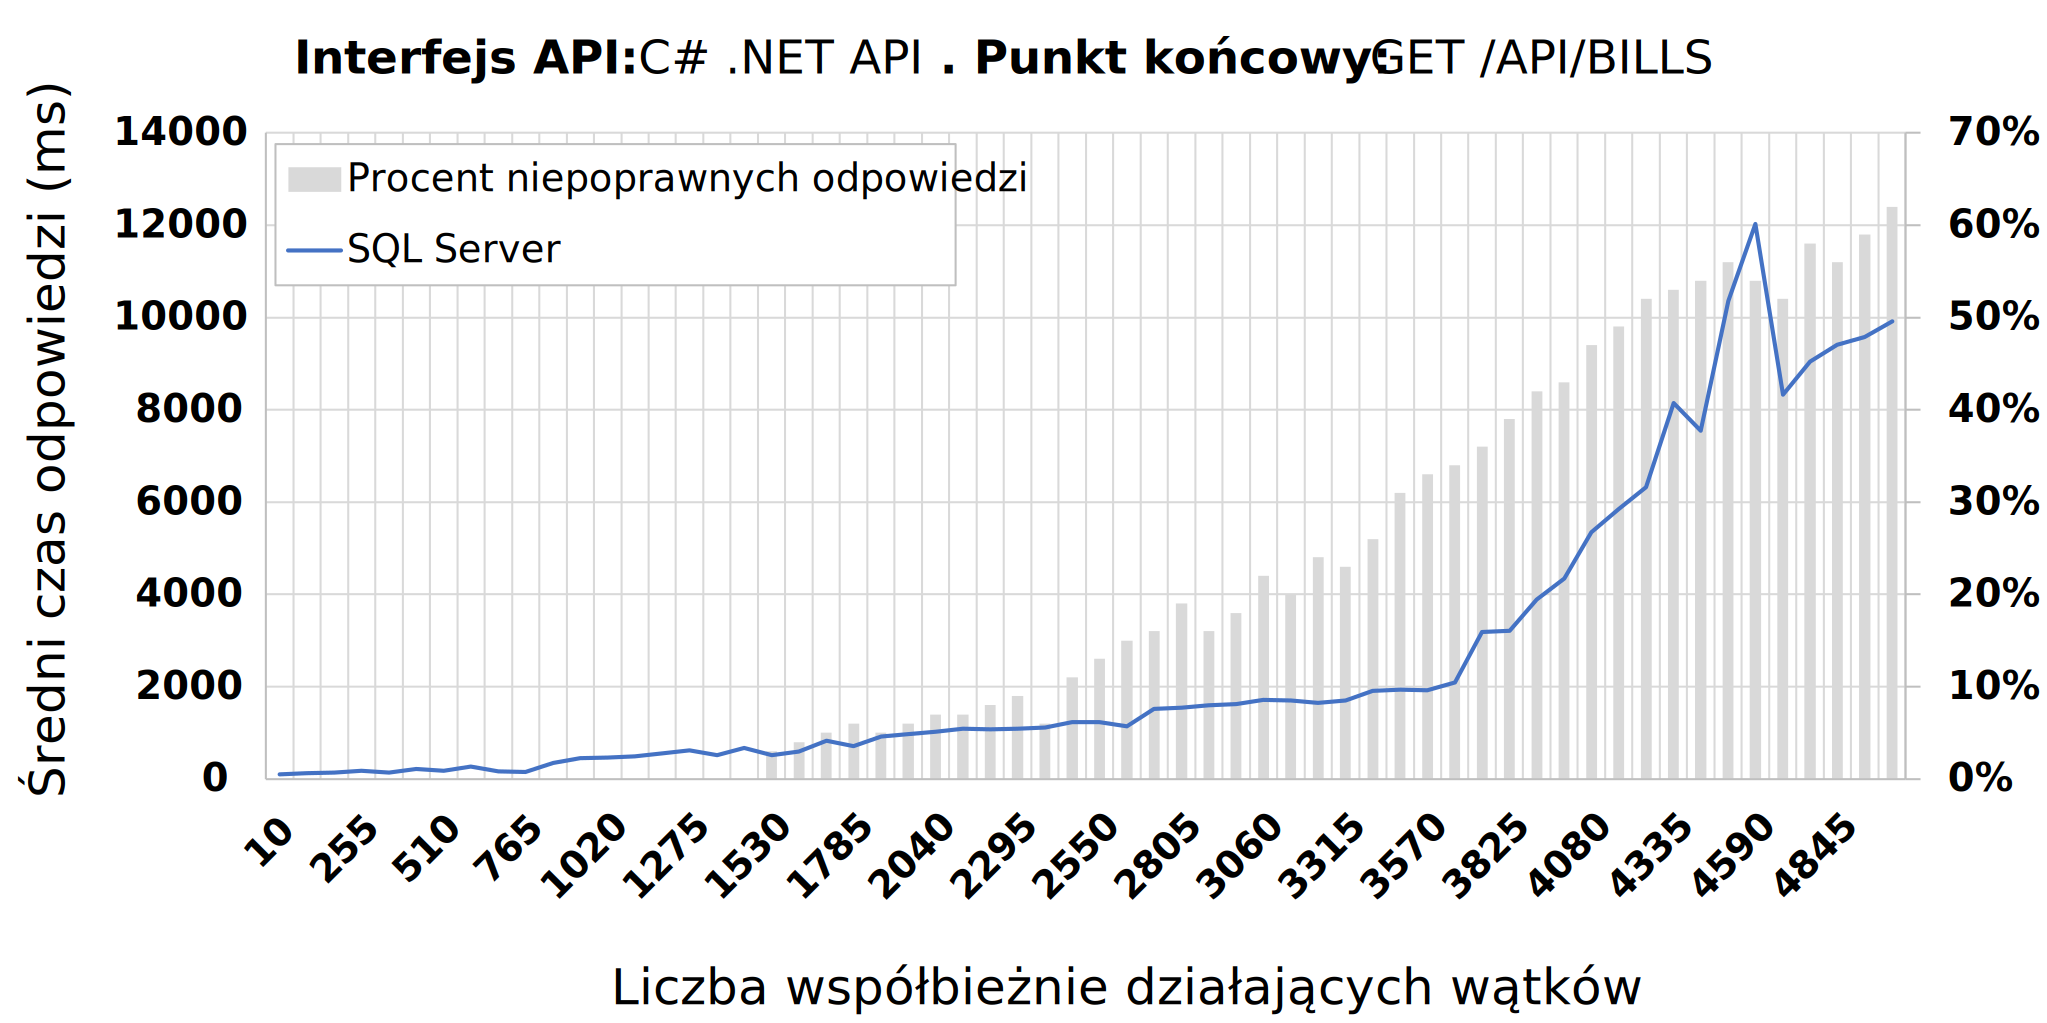
\includegraphics[width=0.49\textwidth]{rys05/response-and-errors-dotnet.pdf} & 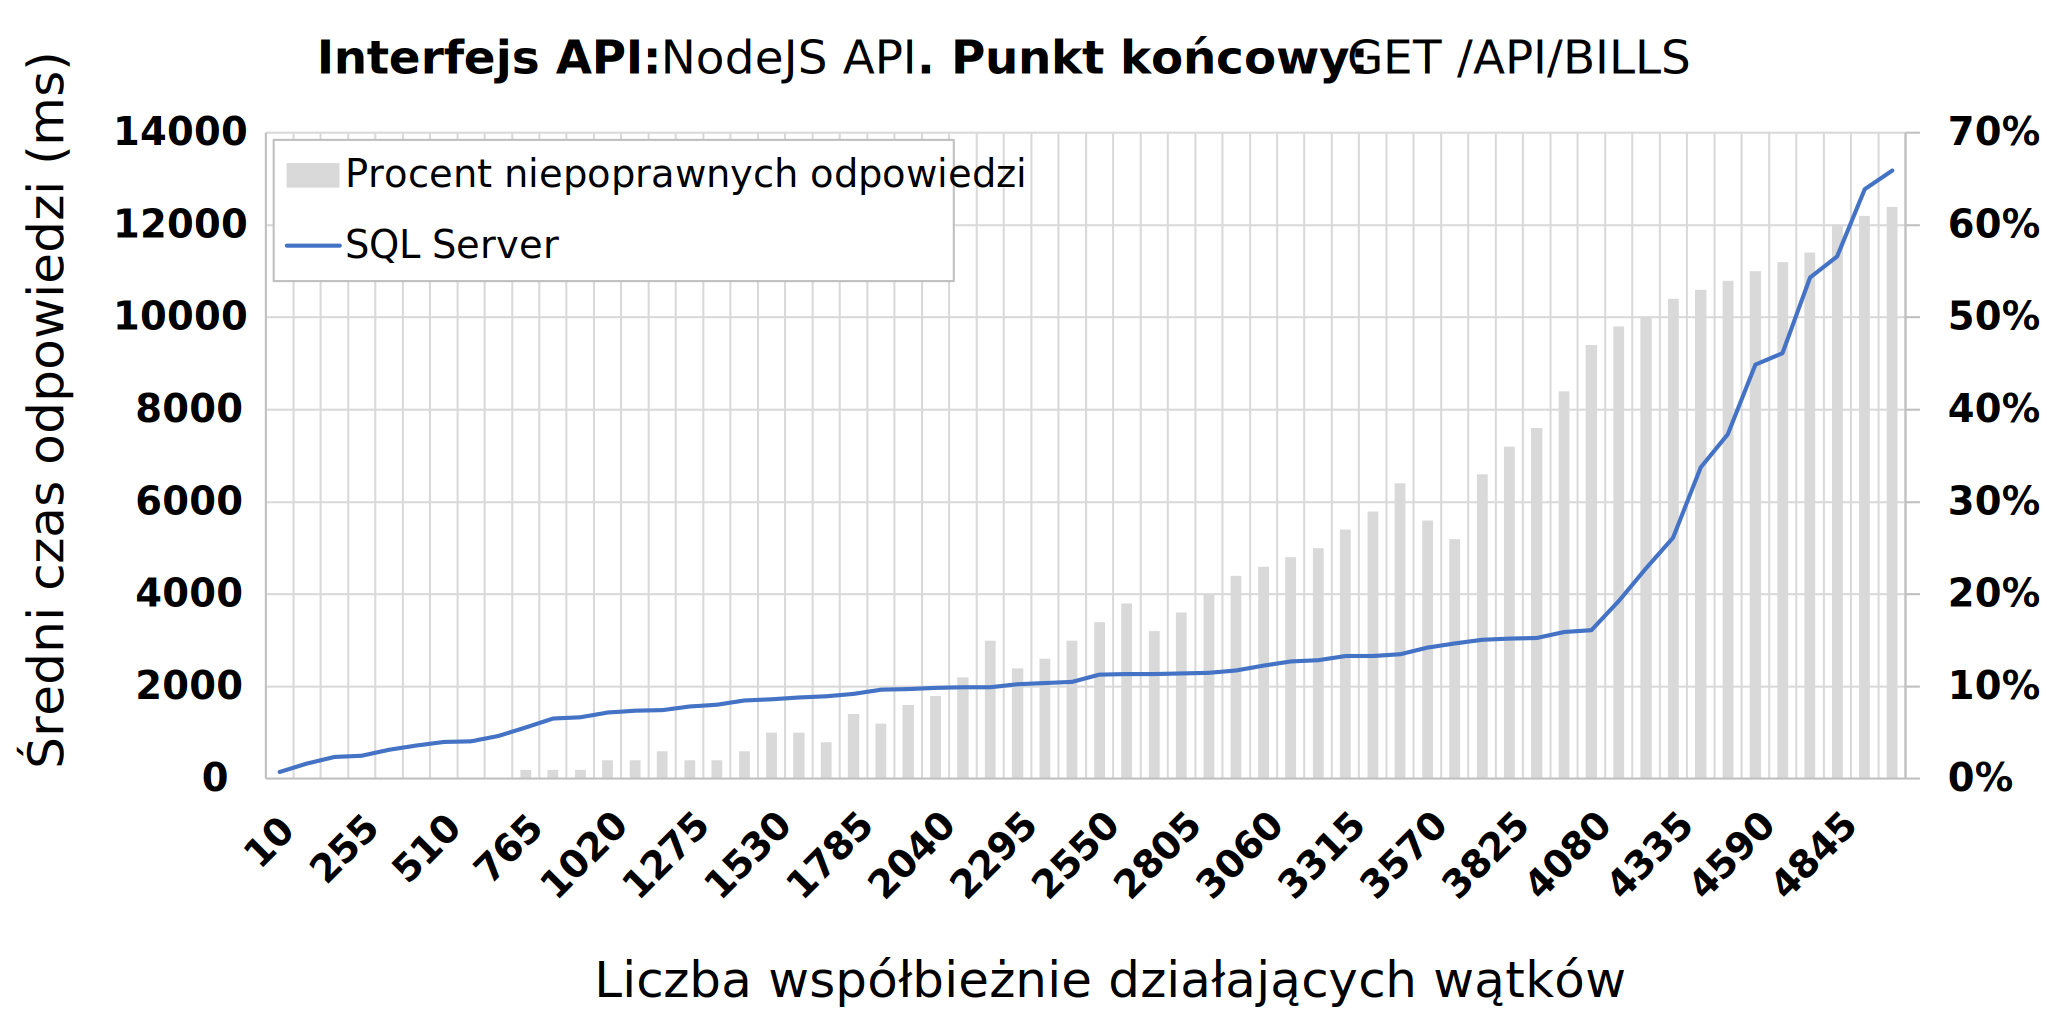
\includegraphics[width=0.49\textwidth]{rys05/response-and-errors-nodejs.pdf}
      % jezeli obraki sa rownej wysokosci, mozna je wyrownac do gory stosujac vtop jak nizej
      % \vtop{\vskip-2ex\hbox{{\includegraphics[width=0.475\textwidth]{rys05/beta1}}}} &
      % \vtop{\vskip-2ex\hbox{{\includegraphics[width=0.475\textwidth]{rys05/alfa1}}}}  \caption{Wyznaczanie trajektorii lotu rakiety: 
      \end{tabular}
    \caption{Średnie czasy odpowiedzi na żądanie oraz procent niepoprawnych odpowiedzi względem liczby procesów generujących}
    \label{fig:response-with-errors}
  \end{figure}

Analizując przedstawione wykresy należy zwrócić uwagę zarówno na moment pojawiania się błędów obsługi żądania, jak i na stopień korelacji błędów z czasem przetwarzania zapytania. W przypadku interfejsu API opartego o technologię .NET widzimy, że procent błędów jest silnie powiązany ze zwiększającym się przedziałem czasowym obsługi komendy, a także intensyfikacją ruchu sieciowego. Oznacza to, że serwer w momencie kolejkowania żądań do przetworzenia, nie bierze pod uwagę ich liczby i stara się przetwarzać każde, jakie do niego dotrze. W związku z odmową realizacji funkcjonalności ze strony API, serwer zgłasza wyjątek protokołu hipertekstowego. Z racji konieczności wykonania pracy w kontekście każdego żądania, niezależnie od niewielkiego prawdopodobieństwa jego pomyślnej realizacji, wydłuża się czas uzyskania odpowiedzi na zapytanie klienckie.

Odnosząc się do interfejsu zaimplementowanego w technologii NodeJS, zaobserwować możemy odmienne zachowanie. Pierwszym aspektem na jaki należy zwrócić uwagę jest pojawienie się błędów obsługi żądania zdecydowanie wcześniej (tj. przy znacząco mniejszej liczbie uruchomionych wątków testowych). Oznacza to, że usługa nie jest w stanie radzić sobie na tyle dobrze z dostarczanym ruchem, jak robi to interfejs napisany w języku C\#. Jednakże, wraz z rosnącym błędem procentowym nie zmienia się czas obsługi żądania. Oznacza to, że komponent serwerowy w ramach API nie przetwarza każdego z zapytań jakie zostanie do niego dostarczone, a także w pewien specyficzny względem swojej charakterystyki sposób, dokonuje wyboru tych spośród otrzymanych żądań, które mają zostać natychmiastowo odrzucone. Taki model przetwarzania komunikatów pozwala na utrzymanie niskiego poziomu czasu odpowiedzi, jednakże należy wziąć pod uwagę fakt, że nie musi być ona jednoznaczna z poziomem wydajności działania API.

Biorąc pod uwagę przedstawione fakty, zdecydowano się na wprowadzenie dodatkowej formy wizualizacji, łączącej ze sobą informacje o czasie odpowiedzi oraz procentowym błędzie. Na podstawie tej fromy wizualizacji możliwa będzie prawidłowa ocena wydajności systemów internetowych, uwzględniając zastosowane systemy bazodanowe.

W tabelach X i Y, odnoszących się kolejno do interfejsu implementowanego w technologii .NET oraz usługi tworzonej za pomocą języka JavaScript, wprowadzono trójelementowe wektory, nazwane przez autora pracy wektorami wydajności.

Poszczególne składowe wektora wydajności odnoszą się kolejno do:
\begin{itemize}
    \item maksymalnej liczby uruchomionych wątków oprogramowania testowego dla których współczynnik APDEX usługi wynosi 1
    \item minimalnej liczby uruchomionych wątków oprogramowania testowego dla których współczynnik APDEX usługi wynosi 0
    \item minimalnej liczby uruchomionych wątków oprogramowania testowego dla których procent niepoprawnych odpowiedzi usługi przekracza 50\%.
\end{itemize}

Tak sformułowane elementy, nie tylko pozwalają na przedstawienie bardziej obiektywnego rezultatu dotyczącego wydajności, ale także niosą ze sobą informacje związaną z podziałem przeprowadzonego testu na fazę ewaluacji bazowej, obciążeniowej oraz przeciążającej.

%% TABELKA
%% NA PODSTAWIE INFO Z TABELI ZE DWA WNIOSKI I MAMY READY

\section{Wpływ zastosowanej technologii programistycznej na wydajność realizacji operacji współbieżnych}
\section{Wpływ zastosowanej technologii programistycznej na efektywność obsługi operacji asynchronicznych}
\section{Wpływ implementacji wzorca projektowego podziału odpowiedzialności na wydajność obsługi żądania klienta}
\label{sec:cqrs-and-database-improvements}
\section{Porównanie efektywności obsługi żądań klienckich w stałym czasie z uwzględnieniem odmienneych implementacji mechanizmów pamięci podręcznej}
\section{Zmienność wydajności interfejsu API wdrożonego na generycznej oraz dedykowanej platformie chmurowej}